\documentclass[12pt]{article}
\usepackage{amsmath} % flere matematikkommandoer
\usepackage{amssymb}
\usepackage[utf8]{inputenc} % æøå
\usepackage[T1]{fontenc} % mere æøå
\usepackage[danish]{babel} % orddeling
\usepackage{verbatim} % så man kan skrive ren tekst
\usepackage[all]{xy} % den sidste (avancerede) formel i dokumentet
\usepackage{graphicx}
\usepackage{listings}
\usepackage{appendix}


\title{Mobil-applikation til administration af webhosting-platform - Surftown\\Projektkursus Systemudvikling 2014\\Delrapport 4}
\date{\today}
\author{Christian Enevoldsen 020691}

\lstset{
  breaklines=true,                 % sets automatic line breaking
}

\begin{document}
\maketitle
\begin{center}
  \textbf{Gruppe}: Simon Warg, Nicklas Warming, Robert Rasmusen
\end{center}
\newpage
\tableofcontents
\newpage
\section*{Indledning}

Denne rapport er skrevet, som dokumentation for den praktiske del af projektkurset "Systemudvikling". Der redegøres for metoder og valg forløbende under og før udvikling. Til at starte med redegøres for formålet og rammerne for projektet, hvor der beskrives om den analysemodel, som er brugt i projektet. Dernæst fokuseres der på kravspecifikation og begrænsninger, efterfulgt af Use cases og Systemdesign. Derefter bliver der redegjort for programtest, user tests, brugergrænsefladen og workflow og afsluttende med en gennemgang af implementeringen og udviklingsprocessen. Til sidst i rapporten er der skrevet et review af artiklen \emph{''Challenges of migrating to Agile methodologies, af Shridhar Nerur, Radhakanta Ma- hapatra og George Mangalara''}. 

\section {IT-Projektet}

\subsection{Formål og rammer}

Det er valgt at bruge ``FACTOR'' \cite{factor} analysen til at specificere rammerne og problemområdet for projektet.
FACTOR anlysen består af de seks nedenstående punkter:
\begin{enumerate}
	\item{\textbf{F}: Beskrivelse af systemfunktionerne til løsning af problemområdet.}	
	\item{\textbf{A}: Beskrivelse af de aktøre, som er indehavere af problemområdet.}
	\item{\textbf{C}: Beskrivelse af forhold, som systemet bliver udviklet under, samt forhold systemet skal bruge. }
	\item{\textbf{T}: Beskrivelse af teknologier, systemet bliver udviklet med, samt systemet i sidste ende vil køre med og kræve.}
	\item{\textbf{O}: Beskrivelse af hovedobjekterne som problemområdet indeholder.}
	\item{\textbf{R}: Beskrivelse af ansvarsområdet for systemet.}

\end{enumerate}
\subsection*{F}
Mobil adgang til udvalgte funktioner, samt Surftowns offentlige info. F.eks. kan en kunde se om en server er nede, og om det påvirker kundens egne services.
\subsection*{A}
Surftowns kunder, der mobilt får mulighed for at tjekke status på servere, samt se status på deres services.
\subsection*{C}
Brugerne skal have IT-kendskab, men ikke nødvendigvis være professionelle eller superbrugere. Surftown har ønsket applikationer til iOS og Android. Udviklingsarbejdet foregår ikke på fuld tid, eftersom det er et studieprojekt.
\subsection*{T}
Android applikationen vil blive udviklet med Google's Android SDK, med deres tilhørende Eclipse plugin. iOS applikationen vil blive udviklet med Apple's Xcode. Udviklingsgrupperne har hver især, resourcer til kørselstest under udviklingen.
\subsection*{O}
Objekterne for problemområdet er beskrevet i sektion \ref{class_diagram_section}
\subsection*{R}
Administrativ værktøj for Surftowns kunder, og kommunikationsmiddel mellem Surftown og deres kunder.

\subsection{Kravspecifikation}
Sammen med Surftown er der besluttet funktionelle og ikke-funktionelle krav, samt begrænsninger til applikationen. Disse krav er vigtige for brugeren, samt specificerede til smartphonebrug. Applikation skal udvikles specifikt til iOS og android (native). Dette er et valg foretaget med Surftown, fordi applikationen skal være hurtig. F.eks skal brugeren ikke vente 2 sekunder på at det første view bliver loaded, hvilket ville være tilfældet, hvis vi hentede hjemmesiden ned og viste tilpasset til smartphonen. 

\subsection*{Funktionelle krav i prioteret rækkefølge}
\label{functionlist}
\begin{enumerate}
  \item{Surftown kontaktoplysninger.}
	\begin{itemize}
		\item{Et simpelt skærmbillede, hvor brugeren kan se Surftowns kontaktoplysninger.}
	\end{itemize}
  \item{En login funktion.}
	\begin{itemize}
		\item{En funktion, der giver brugeren mulighed for at logge ind med e-mail og password.}
	\end{itemize}
  \item{Driftstatus af brugerens webhosting.}
	\begin{itemize}
		\item{En informativ funktion, hvor brugeren kan se opdateringer omkring tekniske fejl hos Surftown, som påvirker brugerens webhosting.}
	\end{itemize}
  \item{Driftstatus af brugerens E-mail hosting.}
	\begin{itemize}
		\item{En informativ funktion, hvor brugeren kan se opdateringer omkring tekniske fejl hos Surftown, som påvirker brugerens email.}
	\end{itemize}
  \item{Driftstatus af brugerens database hosting.}
	\begin{itemize}
		\item{En informativ funktion, hvor brugeren kan se opdateringer omkring tekniske fejl hos Surftown, som påvirker brugerens database hosting.}
	\end{itemize}
  \item{Driftstatus af brugerens webmail.}
	\begin{itemize}
		\item{En informativ funktion, hvor brugeren kan se opdateringer omkring tekniske fejl hos Surftown, som påvirker brugerens webmails.}
	\end{itemize}
  \item{Oversigt over brugt/ledigt plads på brugerens hostings.}
	\begin{itemize}
		\item{En informativ funktion, hvor brugeren kan se hvor meget ledigt plads der er tilbage på brugerens forskellige hostingsservices.}
	\end{itemize}
  \item{Status af brugerens domæner.}
	\begin{itemize}
		\item{En informativ funktion, hvor brugeren har mulighed for at se en oversigt over alle brugerens domæner, som er tilknyttet Surftown, samt relevant information om domænerne.}
	\end{itemize}
  \item{OS type (Windows/Linux) for brugerens webhostings.}
	\begin{itemize}
		\item{En informativ funktion, hvor brugeren kan se hvilke operativsystem som brugerens hostingservices køre.}
	\end{itemize}
  \item{En guide til at sætte Surftowns e-mail oplysninger op på en smartphone.}
	\begin{itemize}
		\item{En simpel side hvor der er en guide i tekst- og billedeform, som beskriver hvordan man sætte en Surftown E-mail konto op på en Android/iPhone telefon.}
	\end{itemize}
  \item{Mulighed for at recover sit bruger password.}
	\begin{itemize}
		\item{En funktion hvor brugeren kan skrive sin E-mail ind for at få tilsendt et nyt password.}
	\end{itemize}
  \item{En oversigt brugerens fakturaer.}
	\begin{itemize}
		\item{En informativ funktion, hvor brugeren kan se en oversigt over de betalte og udestående fakturaer, som brugeren har hos Surftown.}
	\end{itemize}
  \item{Udløbningsdato'er for brugerens domæner.}
	\begin{enumerate}
		\item{En informativ funktion, hvor brugeren kan se hvornår dens domæner, tilknyttet til Surftown skal fornys.}
	\end{enumerate}
  \item{Løbende priser for brugerens domæner.}
	\begin{enumerate}
		\item{En informativ funktion, hvor brugeren kan se hvor meget dens domæner koster per betalingsperiode. (Dette er relevant da .dk, .se, .com osv. har forskellige priser)}
	\end{enumerate}
  \item{Løbende priser for brugerens webhostings.}
	\begin{enumerate}
		\item{En informativ funktion, hvor brugeren kan se faktureringsprisen for hver hosting service, som brugeren har hos Surftown.}
	\end{enumerate}
  \item{Antal tilladte tilknyttede domæner til hver af brugerens webhostings.}
	\begin{enumerate}
		\item{En informativ funktion, hvor brugeren kan se hvor mange domæne Surftown tillader, at tilknytte til brugerens hosting services.}
	\end{enumerate}
  \item{Visning af tilkøbte supportkode}
	\begin{enumerate}
		\item{En informativ funktion, hvor brugeren kan se evt tilkøbte supportkoder.}
	\end{enumerate}
\end{enumerate}
Af de funktionelle krav er prioriteres implementeringen af de første 6 punkter højest. Det er valgt, fordi Surftown prioriterer dem højest.
\subsection*{Ikke-funktionelle krav}
\label{nonfunctionlist}
\begin{enumerate}
  \item{Applikationen skal være brugervenlig og intuitiv at bruge. Her er det vigtigt at sætte fokus på at brugeren føler sig hjemme når de bruger applikationen. F.eks på iOS-versionen er det vedtaget at bruge UINavigationController til navigation i applikationen. Det er standard user experience på iOS apps. Det der kendetegner det er f.eks. " $ < $ Back " knappen, som alle iOS brugere ved hvad gør.}
  \item{Applicationen skal være hurtig. Som skrevet før, er det en mulighed at hente Surftowns hjemmeside ned og vist den pænt, men så ville den ikke være hurtig. Derfor vælges der at implementere applikationerne native til deres styresystem. Der fokuseres også på caching, så anvenderen ikke skal hente de samme data ned fra web-serveren hver gang anvenderen går til et view. F.eks. bliver domæner cachet i et array, så det hurtigt kan vises næste gang domæneviewet bliver vist.}
  \item{Applikationen skal være stabil. Det vil sige ingen eller kun få nedetider og ingen crashes eller fejlmeddelelser. }
\end{enumerate}
\subsection*{Begrænsninger}
\label{constrains}
\begin{enumerate}
  \item{Applikationen skal følge Surftowns officielle design-guidline. Den er ikke tilgængelig for offentligheden}
  \item{Applikationen skal nemt kunne oversættes og undestøtte forskellige sprog [implementeringskrav]}
  \item{Applikationen skal skrives native til Android og iOS [implementeringskrav]}
\end{enumerate}

\subsection*{Klassediagram over problemområdet}
\label{class_diagram_section}
\begin{figure}[h]
	\centering
	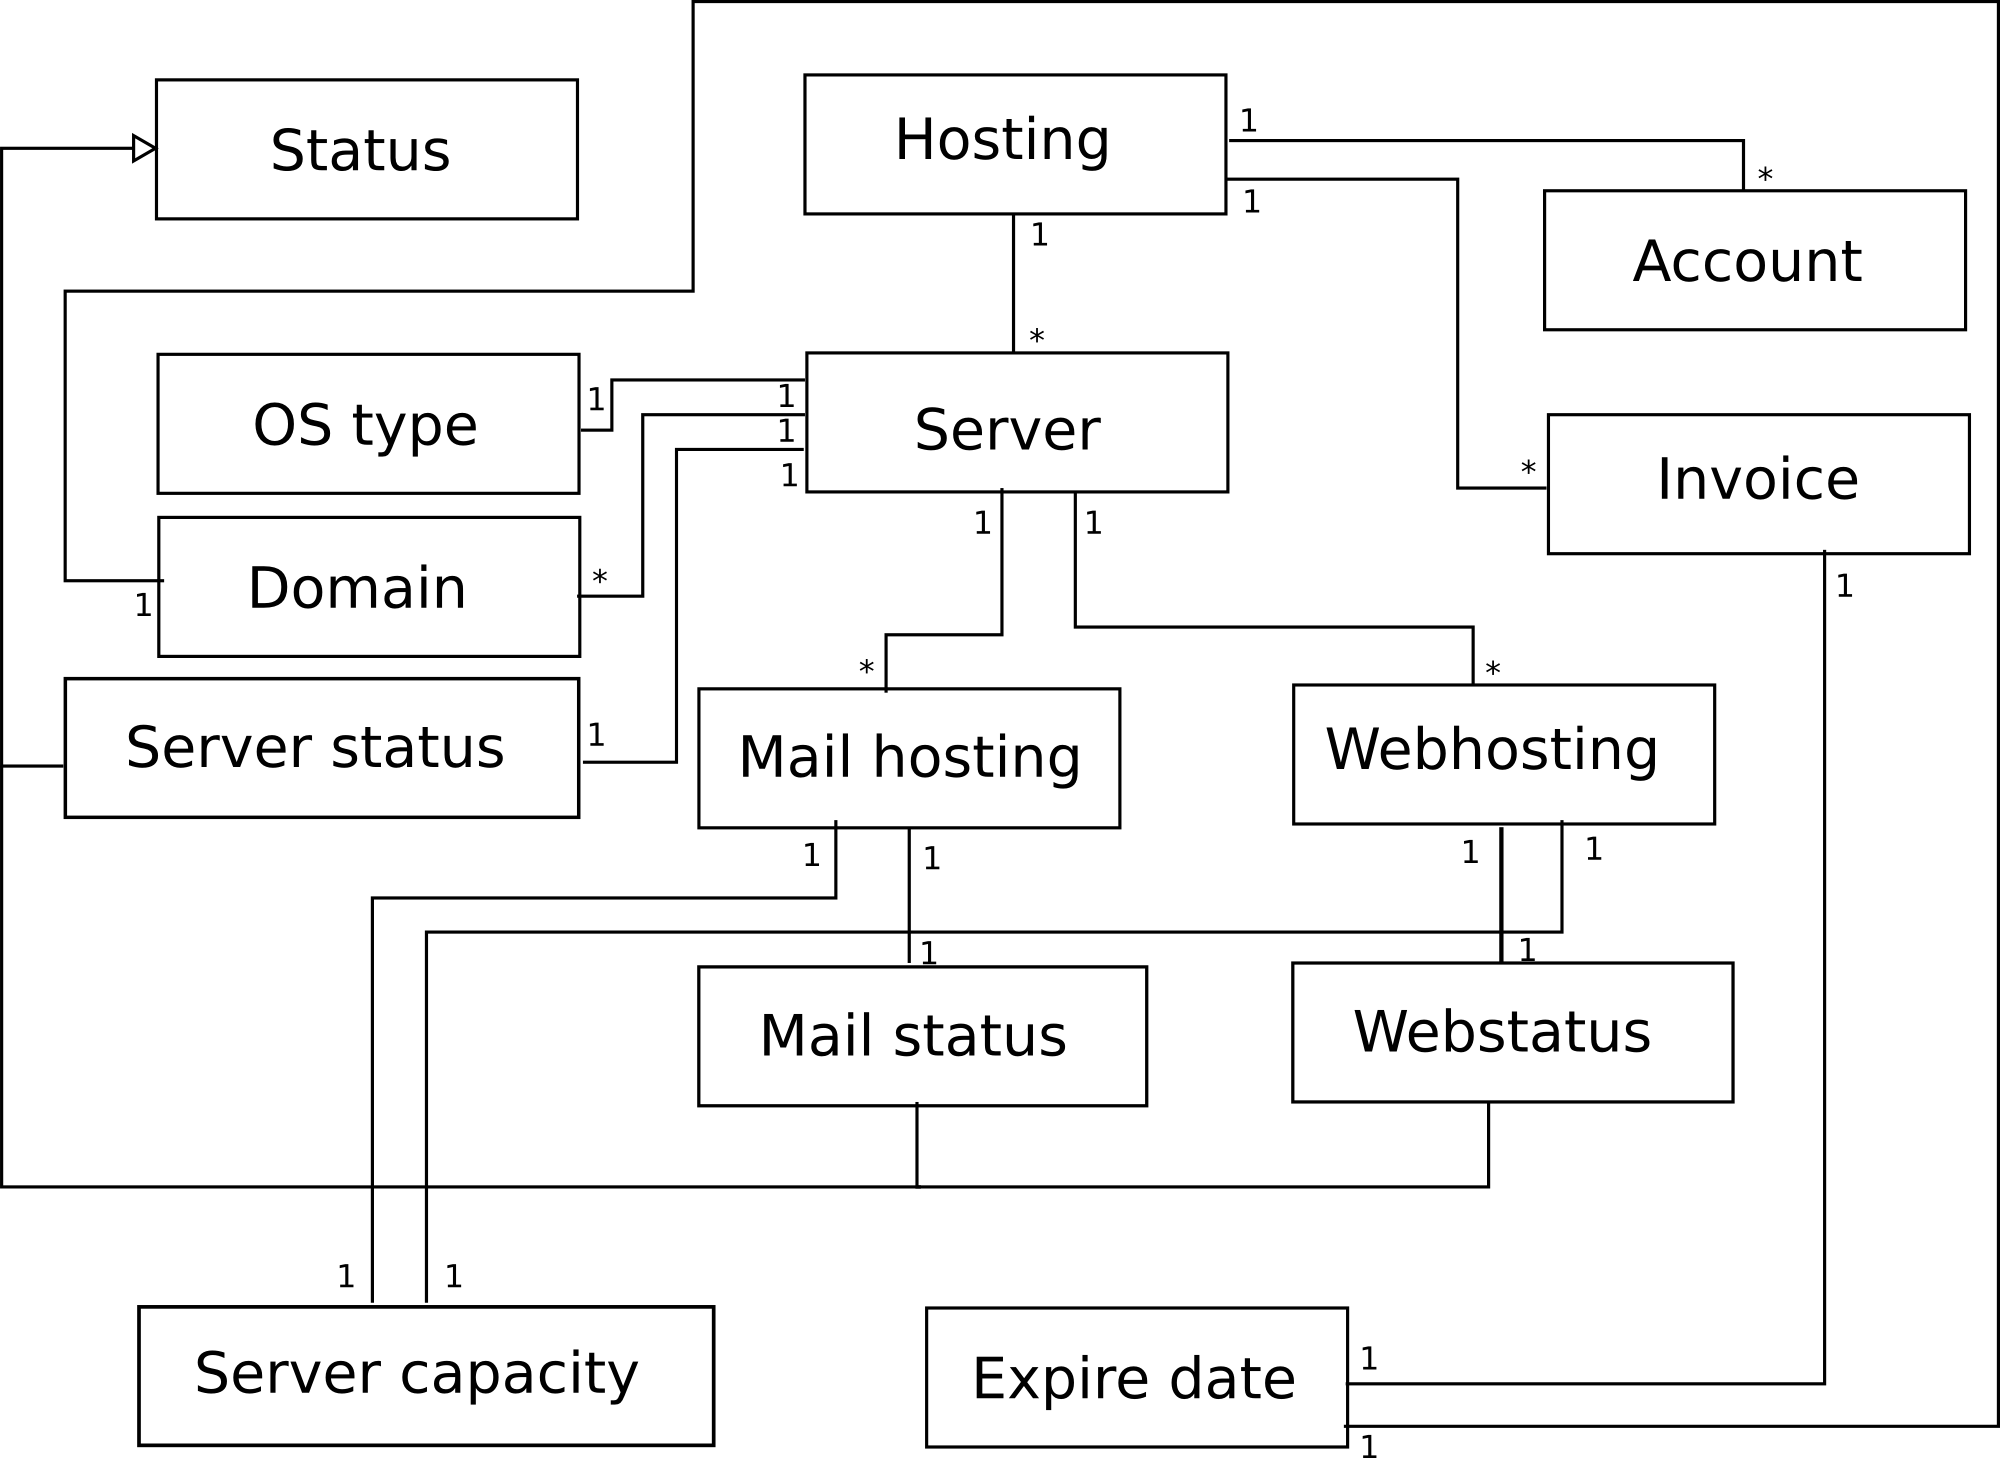
\includegraphics[width=13cm]{class_diagram_v2.png}
	\caption{Figur af klassediagramet over problemområdet}
	\label{classdiagram}
\end{figure}
På figur \ref{classdiagram} ses et klassediagram af problemområdet, inspireret af metoderne beskrevet i kapitel 5 \emph{Analysis} i \cite{OOSE}. 
\begin{enumerate}
	\item{\textbf{Hosting: }Klassen ``Hosting'' fungerer som hovedklassen i diagramet, og er klassen, som repræsenterer det produkt Surftown udbyder, som deres kunder har købt (uafhænigt af servicetypen).}
	\item{\textbf{Account: }For hver ``Hosting'' er der adskillige ``Account'', som repræsenterer de brugere, som er oprettet og har adgang til hosting hos Surftown.}
	\item{\textbf{Invoice: }Da Surftown ikke tilbyder nogle gratis produkter, er der minium èn ``Invoice'' (oprettelsesgebyr)  klasse tilknyttet en ``Hosting'' klasse. ``Invoice'' klassen repræsenterer en faktura fra Surftown.}
	\item{\textbf{Server: }En ``Hosting'' kan have flere forskellige ``Server'''er tilknyttet til sig.
	}\begin{enumerate}
		\item{\textbf{OS type: }Da Surftown både tilbyder serverer med Linux og Windows som operativsystem, har klassen ``Server'' tilknyttet en værdi, der repræsenterer operativsystemet på serveren.}
		\item{\textbf{Domain: }Hver service kan have flere domæner tilknyttet. Domæner udløber, hvorefter de skal fonyes. Selvom at domæner koster penge, antages det at klassen ``Hosting'' tager sig af det, da Surftown sender en samlet regning ud for hver service (Hvilket indbefatter at betale penge for et eller flere domain name(s))}
	\item{\textbf{Web/E-mail hosting: } En server kan have flere web og e-mail -hosting. Både web og email hosting har en kapacitetskvote (``Server Capacity''), som er mængden af data, der kan være på de dem.}
	\end{enumerate}
	\item{\textbf{Super klassen Status og Status(ser)}: } I klassediagrammet på figur~\ref{class_diagram}, kan man se der eksisterer en super klasse kalder ``Status'', som bliver nedarvet fra henholdsvis ``Server status'', ``Mail status'' og ``Web status''. De tre forskellige status klasser nedarver alle fra superklassen ``Status'' da de grundlæggende repræsenterer den samme form for information, men varierer i graden og kvaliteten (forstået som typen) af information.
\end{enumerate}

\subsection*{Use cases og aktører}
Der indgår tre forskellige aktører i systemet; ``User'', ``SurftownProxyAPI'' og ``SurftownAPI'', som henholdvis er følgende:
\begin{enumerate}
	\item{\textbf{User: } Brugeren af applikationen.}
	\item{\textbf{SurftownProxyAPI: } Et middleware (mellemmand) der står for kommunikationen mellem applikationen og Surftown interne API.}
	\item{\textbf{SurftownAPI: } Surftowns interne API, som leverer informationer om brugeren og Surftown.}
\end{enumerate}

\begin{figure}[!h]
	\centering
	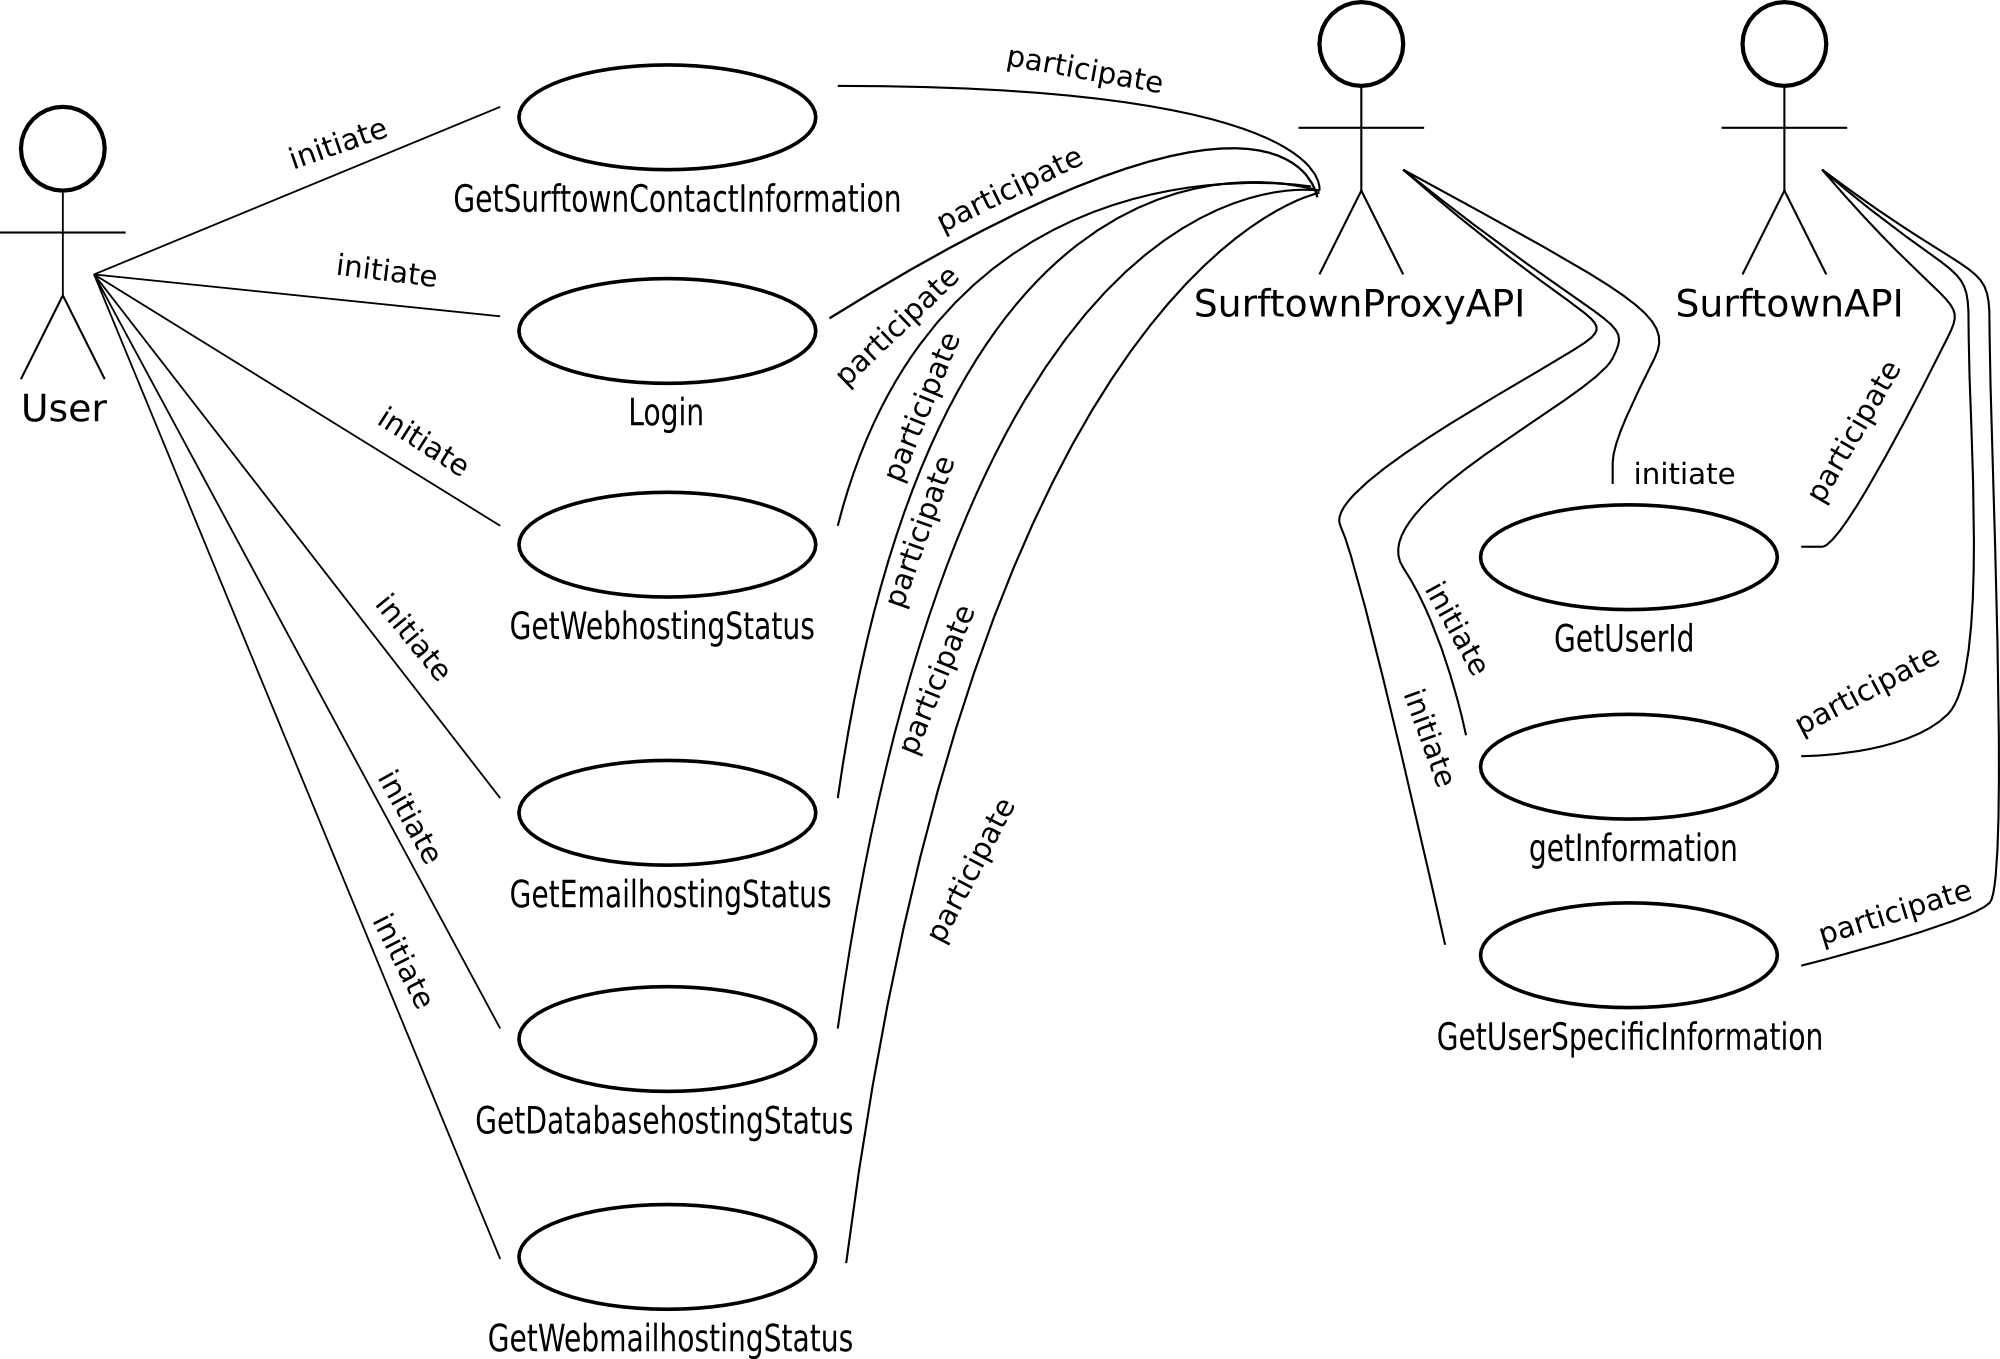
\includegraphics[width=13cm]{high_level_diagramv2.png}
	\caption{Højniveau-diagram af systemet, som beskrevet i \emph{Object-Oriented Software Engineering Using UML, Patterns, and JAVA}\cite{OOSE} kapitel 4.}
	\label{highleveldiagram}
\end{figure}


Figur \ref{highleveldiagram} viser et højniveau-diagram af de seks første funktioner beskrevet i afsnit \ref{functionlist}. Som man kan se på figur \ref{highleveldiagram}, bliver alle funktionerne i figuren som er listet i afsnit \ref{functionlist} startet af aktøren ``User''. De har alle sammen aktøren ``SurftownProxyAPI'' som participater, da alt information fra og til ``User'' går igennem denne aktør.\\Aktøren ``SurftownProxyAPI'' kan starte tre forskellige funktioner, som alle har ``SurftownAPI'' som participater. Disse tre funktioner: ``GetUserId'', ``GetInformation'' og ``GetUserSpecificInformation'' er henholdvis til at, hente et unikt ID, som indentificerer ``User'', hente generel information om Surftown og hente information omhandlende ``User''. 

\subsubsection*{Specificerede use cases}
Som beskrevet i \emph{Object-Oriented Software Engineering Using UML, Patterns, and JAVA}\cite{OOSE} kapitel 4, laves 3 forskellige use cases og deres tilhørende sekvensdiagramer, som dækker de 3 mest interresante funktioner. De første to use cases, og deres tilførende sekvensdiagramer beskriver to forskellige specifikke funktioner, henholdsvis ``RecoverPassword'' (figur~\ref{RecoverPasswordUseCase}~og~\ref{fig:RecoverPassword}) og ``Login'' (figur~\ref{LoginUseCase}~og~\ref{fig:Login}). Den resterende funktion ``GetPrivateInformation'' (figur~\ref{GetPrivateInformationUseCase}~og~\ref{fig:GetPrivateInformation}) beskriver funktionaliteten når brugeren er logget ind.\\\\
I use case figurene [figurer \ref{RecoverPasswordUseCase}, \ref{LoginUseCase}, \ref{GetPrivateInformationUseCase}], er det for simpeltheden skyld, valgt at behandle aktørene ``SurftownProxyAPI'' og ``SurftownAPI'' som èn aktør. Dette er gjort, da ``SurftownProxyAPI'' fungerer som en udvidelse til ``SurftownAPI'', og det således på et ikke-teknisk niveau fungerer som èn aktør. De behandles dog som seperate aktører i sekvensdiagrammerne.

	\hspace{-20pt}
	\rule{430pt}{1.0pt}
	\makebox[100pt][l]{\textbf{Use case navn}} RecoverPassword\\
	\rule{430pt}{0.4pt}
	\makebox[100pt][l]{\parbox{80pt}{\textbf{Deltagende aktøre}}}
	\makebox[100pt][l]{\parbox{\textwidth}{Startet af \textbf{User}\\Kommunikerer med \textbf{Surftown}}}\\
	\rule{430pt}{0.4pt}
	\makebox[100pt][l]{\parbox{80pt}{\vspace{-200pt}\textbf{Event flow}}}
	\makebox[100pt][l]{\parbox{320pt}{
	\begin{enumerate}
	  \item{\textbf{User} aktiverer funktion ``Password recovery'' i applikationen på sin telefon.}
	  \item{Applikationen svare igen ved at vise \textbf{User} en form. Formen består af ét felt hvor \textbf{User} kan angive sin e-mail adresse. Når \textbf{User} har angivet sin e-mail adresse, indsender \textbf{User} formen.}
	  \item{Applikationen modtager formen, og sender \textbf{User} angivet e-mail adresse til \textbf{Surftown}.}
	  \item{\textbf{Surftown} modtager e-mail adressen, og sender en e-mail til e-mail adressen med en vejledning til at genskabe passworded.}
	  \item{\textbf{User} modtager en e-mail, og følger vejledningen.}
	\end{enumerate}
	}}\\
	\rule{430pt}{0.4pt}
	\makebox[100pt][l]{\parbox{80pt}{\textbf{Resultat}}}
	\makebox[100pt][l]{\parbox{\textwidth}{\textbf{User} får nyt password}}\\\rule{430pt}{0.4pt}
\vspace{-30pt}
\begin{figure}[!h]
	\caption{Figuren viser et use-case-diagram af ``RecoverPassword``. ''RecoverPassword`` er en funktion som aktøren  ''User``, brugeren af applikationen, kan aktiverer ved at trykke på en knap, i tilfælde af at brugeren har glemt sine loginoplysninger til Surftown. Når aktøren ''User`` aktiverer denne funktion, viser applikationen en udfyldelses-form, hvor ''User`` kan indtaste og indsende sin E-mail adresse til Surftown. Hvis ''User``'s indtastede E-mail adresse er genkendt af Surftown, vil Surftown sende nye loginoplysninger til aktøren ''User``.}
	\label{RecoverPasswordUseCase}
\end{figure}\\

\begin{figure}[!h]
	\centering
	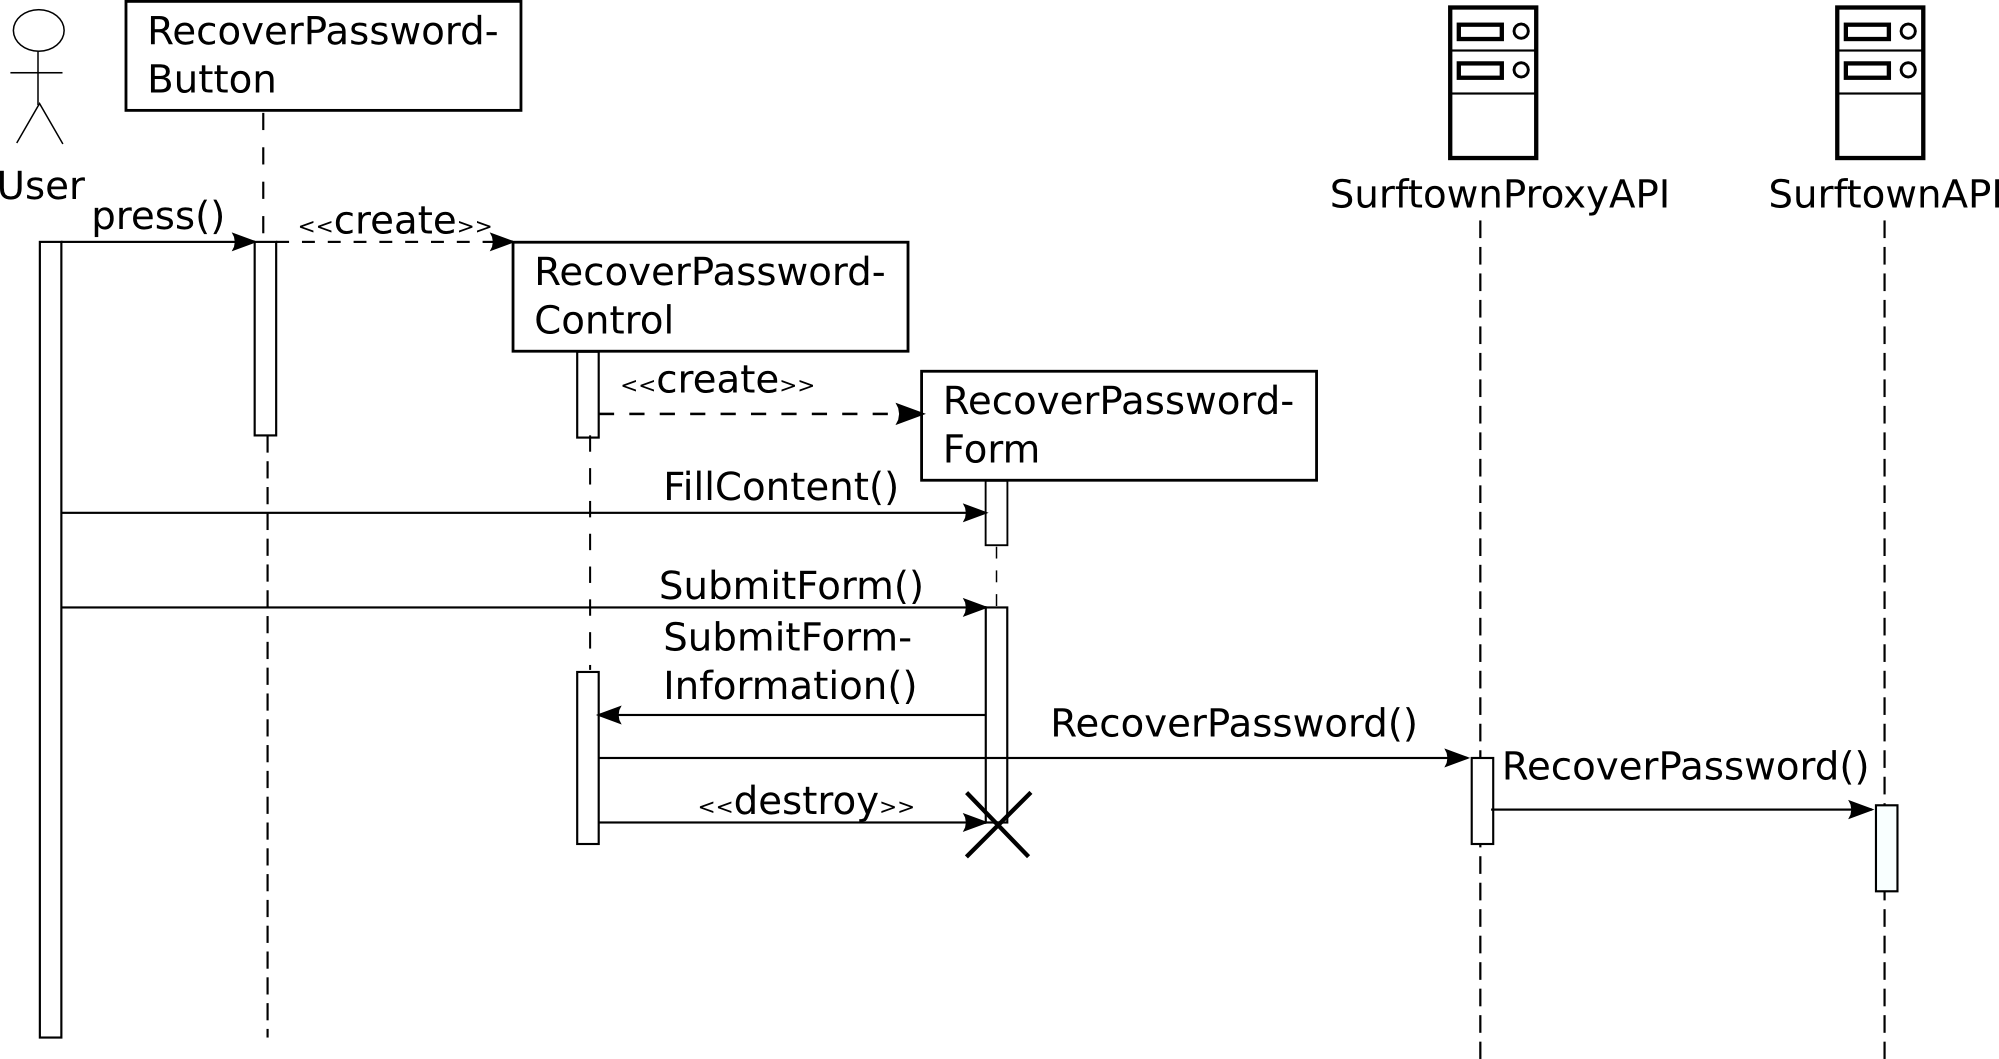
\includegraphics[width=13cm]{sekvens_diagrammer/recoverPassword.png}
	\caption{Figuren viser et sekvensdiagram af ''RecoverPassword`` funktionen, hvis use case er afbilledet i figur \ref{RecoverPasswordUseCase}. I denne figur er alle tre forskellige aktører vist. Det starter med at aktøren ''User`` aktiverer funktionen ''RecoverPassword`` ved at trykke på en knap. Herefter bliver der oprettet et ''RecoverPassword`` objekt, som opretter en boundary, i form af en udfyldelses form, hvor ''User`` kan indtaste information og indsende det. Når ''User`` har indsendt informationen, modtager ''RecoverPassword`` objektet informationen og destruerer den sidste boundary. Herefter sender ''RecoverPassword`` objektet informationen  videre til aktøreren ''SurftownProxyAPI``, som sender det til ''SurftownAPI``, hvorefter ''SurftownAPI`` sørger for at sende nye login-informationer til ''User``.}
	\label{fig:RecoverPassword}
\end{figure}
\newpage
	\hspace{-20pt}
	\rule{430pt}{1.0pt}
	\makebox[100pt][l]{\textbf{Use case navn}} Login\\
	\rule{430pt}{0.4pt}
	\makebox[100pt][l]{\parbox{80pt}{\textbf{Deltagende aktøre}}}
	\makebox[100pt][l]{\parbox{\textwidth}{Startet af \textbf{User}\\Kommunikerer med \textbf{Surftown}}}\\
	\rule{430pt}{0.4pt}
	\makebox[100pt][l]{\parbox{80pt}{\vspace{-285pt}\textbf{Event flow}}}
	\makebox[100pt][l]{\parbox{320pt}{
	\begin{enumerate}
	  \item{\textbf{User} aktiverer funktion ``Login'' i applikationen på sin telefon.}
	  \item{Applikationen svare igen ved at vise \textbf{User} en form. Formen består af to felter hvor \textbf{User} kan angive sin e-mail adresse og password. Når \textbf{User} har angivet sin e-mail adresse og password, indsender \textbf{User} formen.}
	  \item{Applikationen modtager formen, og sender \textbf{User} angivet e-mail adresse og password til \textbf{Surftown}.}
	  \item{\textbf{Surftown} modtager e-mail adressen og passworded, og tjekker gyldigheden af e-mail adressen og passworded. Hvis gyldigt event 5 ellers event 6.}
	  \item{Applikationen logger \textbf{User} ind. \textbf{User} henter sine private informationer fra \textbf{Surftown}, med use casen ``getPrivatInformation''.}
	  \item{Applicationen indikerer overfor \textbf{User} om at \textbf{User} ikke er blevet logget ind, og sender \textbf{User} til event 2 i use case ``Login''.}
	\end{enumerate}
	}}\\
	\rule{430pt}{0.4pt}
	\makebox[100pt][l]{\parbox{80pt}{\textbf{Resultat}}}
	\makebox[100pt][l]{\parbox{\textwidth}{\textbf{User} er logget ind}}\\
	\rule{430pt}{0.4pt}
\vspace{-30pt}
\begin{figure}[!h]
	\caption{Figuren viser et use-case-diagram af Login. ``Login'' er en funktion, som giver aktøren ``User'' mulighed for at se sine private oplysninger, ved at angive sin E-mail og password, som er registreret hos Surftown.}
	\label{LoginUseCase}
\end{figure}\\
\begin{figure}
	\centering
	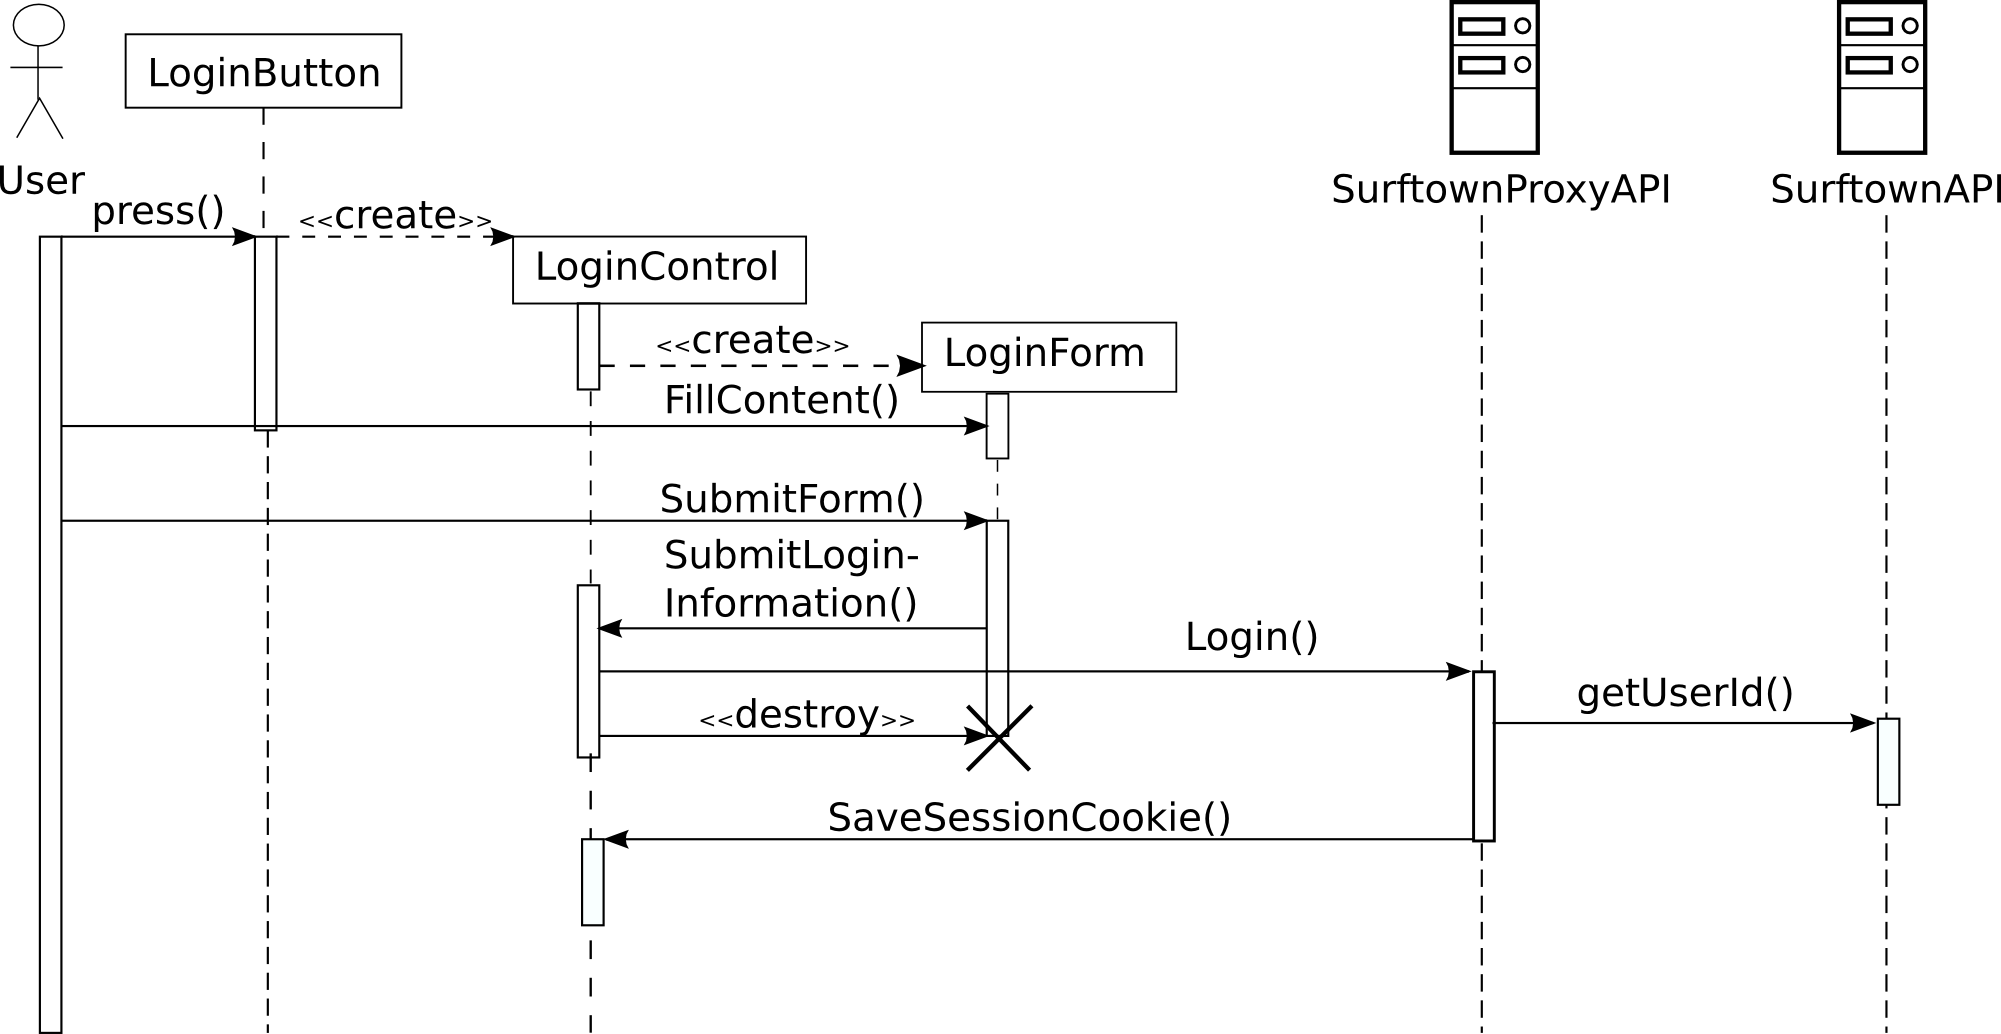
\includegraphics[width=13cm]{sekvens_diagrammer/login.png}
	\caption{Figuren er et sekvensdiagram af ``Login`` funktionen, hvis use case er afbilledet i figur \ref{LoginUseCase}. I denne figur er alle tre forskellige aktøre vist. Aktøren ''User`` aktiverer ''Login`` funktionen, hvorefter et ''Login`` objekt bliver dannet. ''Login`` objektet opretter en login-form boundary, hvor brugeren kan udfylde sine login oplysninger og indsende dem. Når ''User`` indsender oplysningerne, modtager ''Login`` objektet dem, hvorefter ''Login`` objektet sender oplysningerne til aktøren ''SurftownProxyAPI``, samt destruerer login-form boundary'en. ''SurftownProxyAPI`` sender oplysningerne til ''SurftownAPI`` og modtager et user-id, hvorefter ''SurftownProxyAPI`` laver en session-cookie som ''Login`` objektet gemmer. Brugeren er nu logget ind.}
	\label{fig:Login}
\end{figure}

\newpage
	\hspace{-20pt}
	\rule{430pt}{1.0pt}
	\makebox[100pt][l]{\textbf{Use case navn}} getPrivatInformation\\
	\rule{430pt}{0.4pt}
	\makebox[100pt][l]{\parbox{80pt}{\textbf{Deltagende aktøre}}}
	\makebox[100pt][l]{\parbox{\textwidth}{Startet af \textbf{User}\\Kommunikerer med \textbf{Surftown}}}\\
	\rule{430pt}{0.4pt}
	\makebox[100pt][l]{\parbox{80pt}{\vspace{-105pt}\textbf{Event flow}}}
	\makebox[100pt][l]{\parbox{320pt}{
	\begin{enumerate}
	  \item{\textbf{User} beder om sine private informationer.}
	  \item{Applikationen tjekker om \textbf{User} er logget ind. Hvis \textbf{User} er logget ind event 3 ellers event 4}
	  \item{Applikationen henter de private informationer fra \textbf{Surftown} og fremstiller dem for \textbf{User}.}
	  \item{Applikationen kalder use case ``Login''}
	\end{enumerate}
	}}\\
	\vspace{-10pt}
	\rule{430pt}{0.4pt}
	\makebox[100pt][l]{\parbox{80pt}{\vspace{20pt}\textbf{Start betingelse}}}
	\makebox[100pt][l]{\parbox{320pt}{\textbf{User} er logget ind.}}\\
	\rule{430pt}{0.4pt}\\
	\makebox[100pt][l]{\parbox{80pt}{\textbf{Resultat}}}
	\makebox[100pt][l]{\parbox{\textwidth}{\textbf{User} bliver præsenteret for fortrolig information}}\\
	\rule{430pt}{0.4pt}
\vspace{-30pt}
\begin{figure}[!h]
	\caption{Figuren er et use-case-diagram af ``GetPrivateInformation'' funktionen. ``GetPrivateInformation''  Denne funktion bliver kaldt når brugeren skal se ikke-offentlige tilgængelige informationer (f. eks. informationer om brugerens services hos Surftown)}
	\label{GetPrivateInformationUseCase}
\end{figure}\\
\begin{figure}
	\centering
	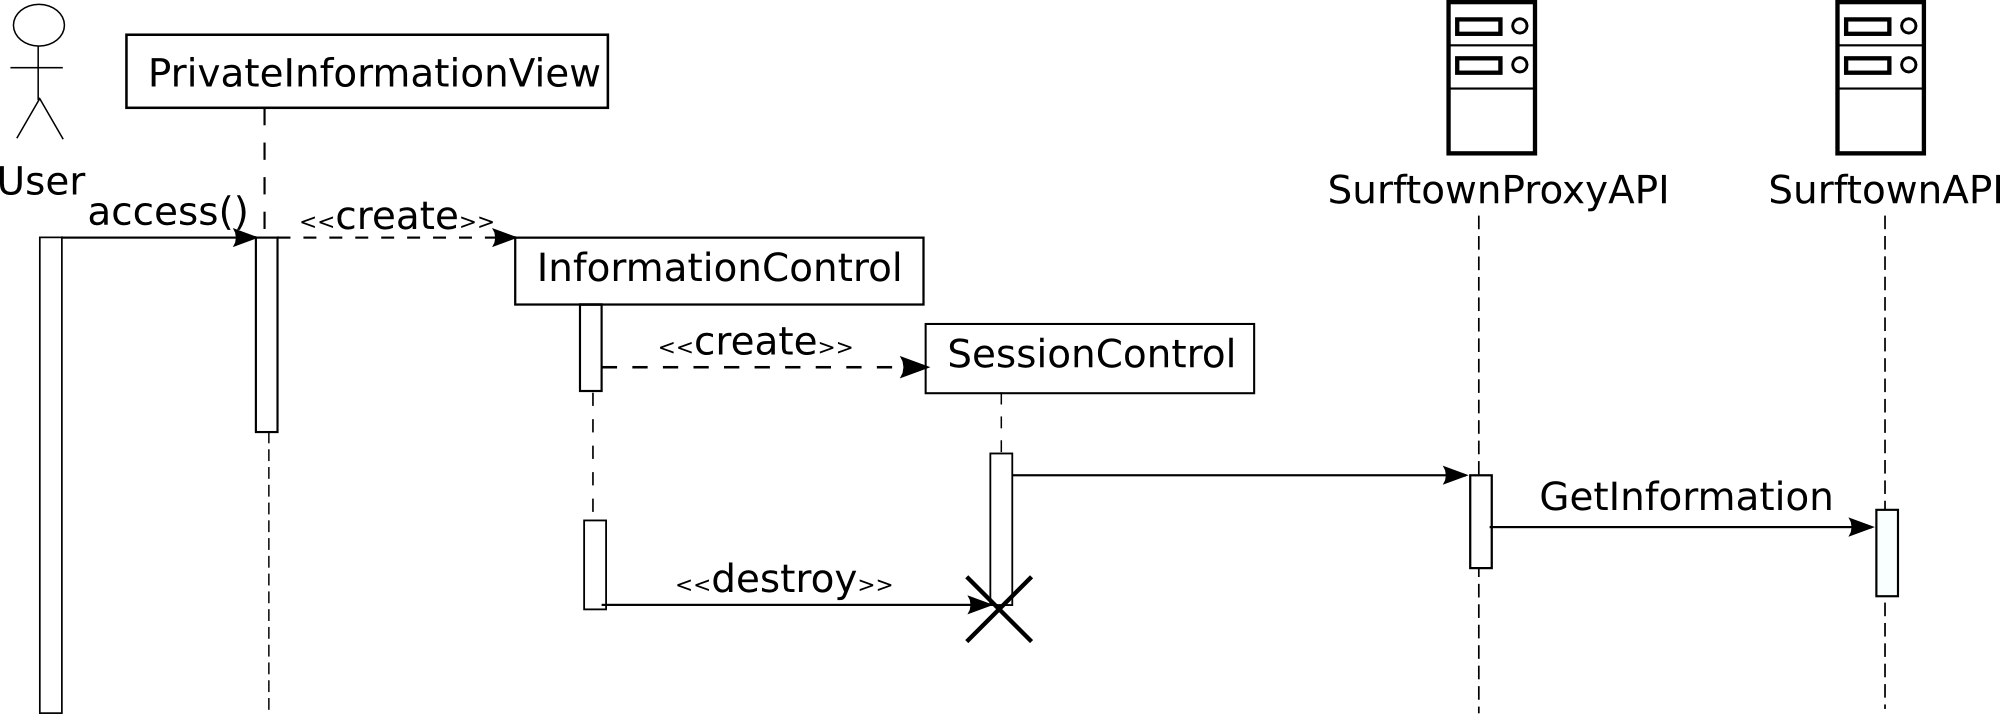
\includegraphics[width=13cm]{sekvens_diagrammer/GetPrivateInformation.png}
	\caption{Figuren er et sekvensdiagram af ``GetPrivateInformation'' funktionen. Funktionen ``GetPrivateInformation'' bliver kaldt når aktøren ``User'' tilgår et view med bruger privat information. Når funktionen bliver kaldt bliver et ``InformationControl'' objekt oprettet, som opretter et ``SessionControl'' objekt. ``SessionControl'' objektet sender en session-cookie (som er optaget via ``Login'' funktionen) til aktøren ``SurftownProxyAPI''. ``SurftownProxyAPI'' beder om de private informationer for ``User'' via et user-id som er associeret med session-cookien.}
	\label{fig:GetPrivateInformation}
\end{figure}
\newpage
\subsection{Systemdesign}
\subsection*{Surftown API}
Surftowns API kaldes via HTTP, og via en bestemt GET variable ``call'' kan man sætte hvilken funktion man vil kalde\footnote{Afhængig af hvilken funktion man kalder, kan man også sætte andre GET variabler.}. 
Men da Surftowns API er designet til at blive brugt på et lokalt netwærk, understøtter API'et ikke nogle former for handlings- eller informationsrestriktioner\footnote{Dette var ellers blevet lovet af Surftown at de ville lave, i forbindelse med udviklingen af dette system}. Det blev derfor nødvendigt at lave en udvidelse af Surftowns API.\\
Resultatet blev til en API proxy server, som er skrevet i Javascript og bliver kørt i NodeJS\footnote{En javascript-baseret server, bygget på Google Chrome's V8 motor}. API proxy serveren understøtter handlings- og informationsrestriktioner med bruger-login og cookie-session, via HTTP protokollen. Det fungerer ved at API proxy serveren kun tillader udvalgte funktioner at blive kaldt, og videresender informationerne til Surtowns API. Hvis en funktion som parameter kræver et bruger-id, vil API proxy serveren tjekke om der er sendt en gyldig session-cookie med i HTTP-requesten, hvis det er tilfældet vil proxy API serveren sende requesten videre sammen med bruger-id'et associeret med session-cookien.

\subsection*{Applikationen}
\begin{figure}[h]
	\centering
	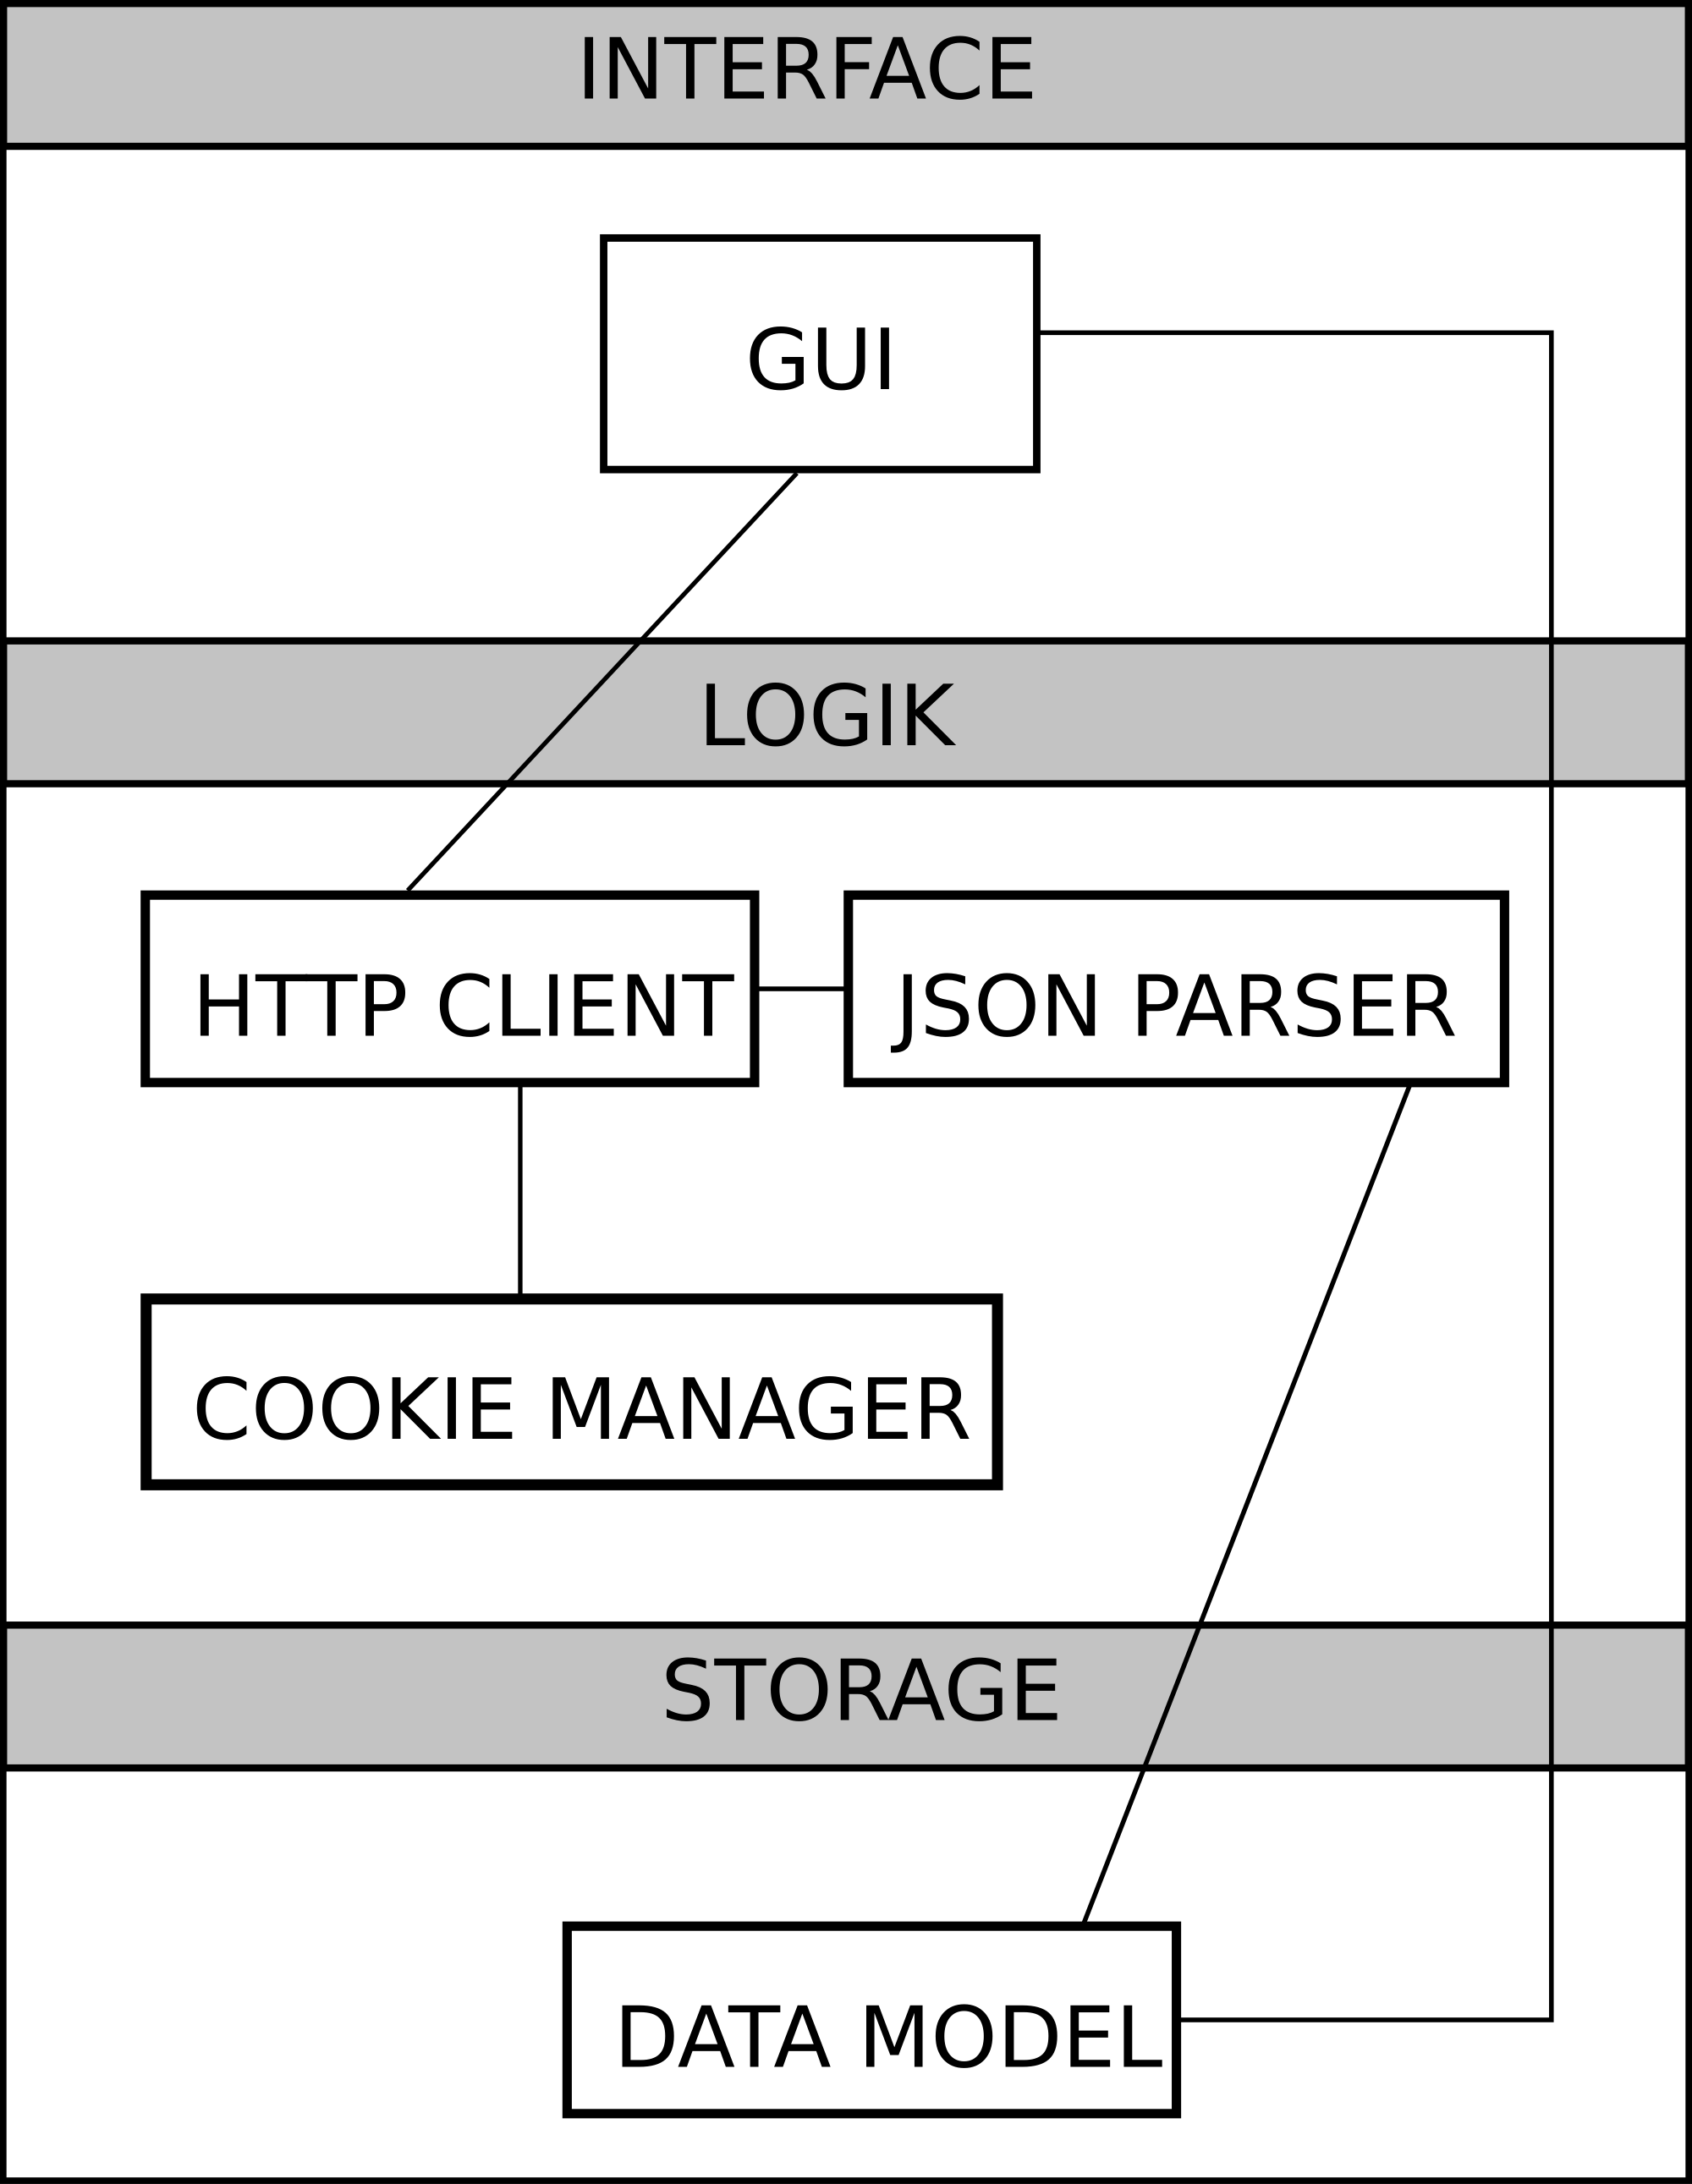
\includegraphics[width=7cm]{system_components.png}
	\caption{Decomposition diagram af applikationen, inspireret af \emph{Object-Oriented Software Engineering Using UML, Patterns, and JAVA}\cite{OOSE}}
	\label{system_components}
\end{figure}
\begin{itemize}
	\item{\textbf{GUI\footnote{Graphical User Interface}: } GUI'en er implementeret sådan at ved ``View'' skifte, dvs. ved nyt skærmbillede, forespørger GUI'en nye data fra  HTTP CLIENT'en og fremviser herefter de data der er i DATA MODEL.}	
	\item{\textbf{HTTP CLIENT: } Ved et request fra GUI'en, laver HTTP CLIENT en request til COOKIE MANAGER, for at få evt. cookies fra en tidligere HTTP request, herefter sender HTTP CLIENT en HTTP request til Surftown API'et og sender de modtaget data til JSON PARSER}	
	\item{\textbf{JSON PARSER: }Når JSON PARSER modtager data vil den dekode dataene og sende de dekodet data til DATA MODEL.}
	\item{\textbf{COOKIE MANAGER: }COOKIE MANAGER sørger for at gemme eventuelle cookies fra tideligere HTTP request, og leverer dem til HTTP CLIENT ved afsendelse af en ny HTTP request. Derudover kontrollerer COOKIE MANAGER cookies'nes udløbstider}
	\item{\textbf{DATA MODEL: }DATAMODEL sørger for at udfylde foruddefineret datastrukturer med de nye data. Dette sørger for at data'ene forbliver konsistente overfor GUI'et, som skal fremvise dem.}
\end{itemize}
\subsection*{Manglende implementeringer}
I afsnit \ref{functionlist} udtrykkedes et ønske om at implementerer de første seks punkter som et minimum, hvilket der ikke blev nået. Der mangler stadig at implementeres:
\begin{enumerate}
	\item Driftstatus af brugerens E-mail hosting.
	\item Driftstatus af brugerens database hosting.
	\item Driftstatus af brugerens webmail
\end{enumerate}
Derudover mangles at implementerer Suftowns officielle design, som er en begrænsning i afsnit \ref{constrains}.


\subsection{Programtest og resultater}
For at være sikker på at systemet er nemt og intuitivt, er der blevet foretaget nogle usability test sammen med en test bruger ``User''\footnote{Simon Warg's sambo}. ``User'' har allereder en hjemmeside hos en anden hosting leverandør end Surftown, men ser ikke sig selv som en erfaren- eller superbruger.\\
Målet med testene er at finde fejl, hvor systemet opfører sig anderledes end forventet specificeret ud fra use case'ene.\\
Fra \emph{Object-Oriented Software Engineering Using UML, Patterns, and JAVA}\cite{OOSE} kapitel 11, er det beskrevet at idèen med usability test, ikke er at vise at systemet ikke indeholder nogle fejl eller bugs, men at forbedre måden systemet bruges på. Derfor er der også foretaget programtest af login, domæne og service funktionaliteterne samt user-experience. Der er ikke foretaget nogle unit-tests. Dette skyldes at udviklere har prioriteret det fra, da kørselstest er rigeligt for de funktioner vi har implementeret. I kørsel bliver funktionerne testet kronologisk, og det ville være dobbeltarbejde at køre unit-tests først, efterfulgt af samme procedure samtidig med at man tester for semantiske, grafiske og user-experience fejl.

\subsection*{Resultat}
Brugeren ''operatøren'' bliver informeret om sin rolle og sine mål som han skal opnå ved at bruge applikationen, som beskrevet i bilag \ref{testSpec}.\\
        \rule{430pt}{1.0pt}
        \makebox[100pt][l]{\textbf{Logge ind:}}
        \makebox[100pt][l]{\parbox{\textwidth}{Brugeren tastede sit brugernavn og password ind,\\ og klikkede på ``Login'' knappen.
                                                                        Brugeren nåede målet.}}\\
        \rule{430pt}{0.4pt}
        \makebox[100pt][l]{\textbf{Finde services:}}
        \makebox[100pt][l]{\parbox{\textwidth}{Brugeren klikkede på ``Services'' i menuen. Han blevet spurgt \\ hvor mange services han kunne se. Det første svar lød på spørgsmålet om, hvad type af service han skulle vælge. \\ Efter en kort forklaring blevet det klart for \textbf{User} at han havde 3 services som  var listet på skærmen. brugeren nåde sit mål}}\\
	\hspace{-20pt}
        \rule{430pt}{0.4pt}
        \makebox[100pt][l]{\textbf{Finde domains:}}
        \makebox[100pt][l]{\parbox{\textwidth}{Brugeren klikkede på ``Home'' fra den nuværende ``Service'' og \\ klikkede bagefter på ``Domains'' i hovedmenuen. Han blevet spurgt hvor mange \\ domæner han kunne se. Han kunne se 3 domæner, hvilket ikke var korrekt. \\ Han blev gjort opmærksom på, at der burde være flere domæner, og spurgte hvad han vil gøre for at finde de resterende. Han klikkede på ``Home'' og gik ud i hovedmenuen, hvorefter han gik ind i ``Domains'' igen. I andet forsøg fandt han ud af at man kunne scrolle for at se de resterende domæne, og han svarede 7, hvilket var korrekt. Brugeren nåede sit mål}}\\

	\hspace{-20pt}
        \rule{430pt}{0.4pt}
        \makebox[100pt][l]{\textbf{Password reset:}}
        \makebox[100pt][l]{\parbox{\textwidth}{\textbf{User} klikkede på ``Forgot password'' på login-skærmen,\\hvorefter et nyt stykke papir blev fremlagt på bordet. \textbf{User} ``tastede'' sin e-mail ind og klikkede på ``Send''. Brugeren nåede sit mål.}}\\

\subsection*{Resultat diskusion}
Det er væsentligt at nævne at der skulle have været foretaget flere user-tests før at resultatet ville være overbevisende. Udover at den kandidat vi har valgt, ville det være åbentlyst også at have inkluderet nogle udvalgte kunder hos Surftown, som i sidste ende er dem der kommer til at bruge applikationen 

\subsection*{Resultat konklusion}
Testene af systemet gik overordnet godt, og brugeren havde ikke de store problemer med at finde de forskellige informationer og funktioner. Dog var der enkelte terminologiske problemer for brugeren, men da terminologien er taget direkte fra Surftowns eksisterende kontrolpanel, er det besluttet at det ikke der skal ændres. 

\subsection{Brugergrænseflade og workflow}
\subsection*{Skærmbilleder}
De følgende billeder, er forskellige skærmbilleder af de vigtigste dele af applikationen på Android og iOS. Dataene som er vist på billederne er data som Surftown har oprettet, på den test server de har stillet til rådighed til projektet.
\newpage
\begin{figure}[h]
	\centering
	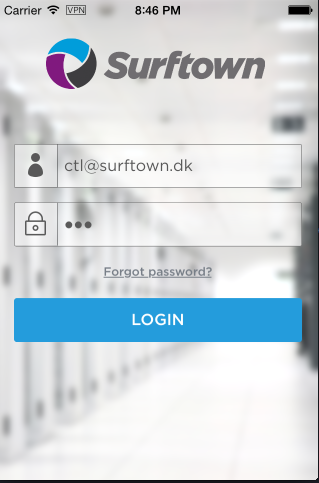
\includegraphics[width=7cm]{ios/login.png}
	\caption{Loginskærm på iOS}
\end{figure}
\newpage
\begin{figure}[h]
	\centering
	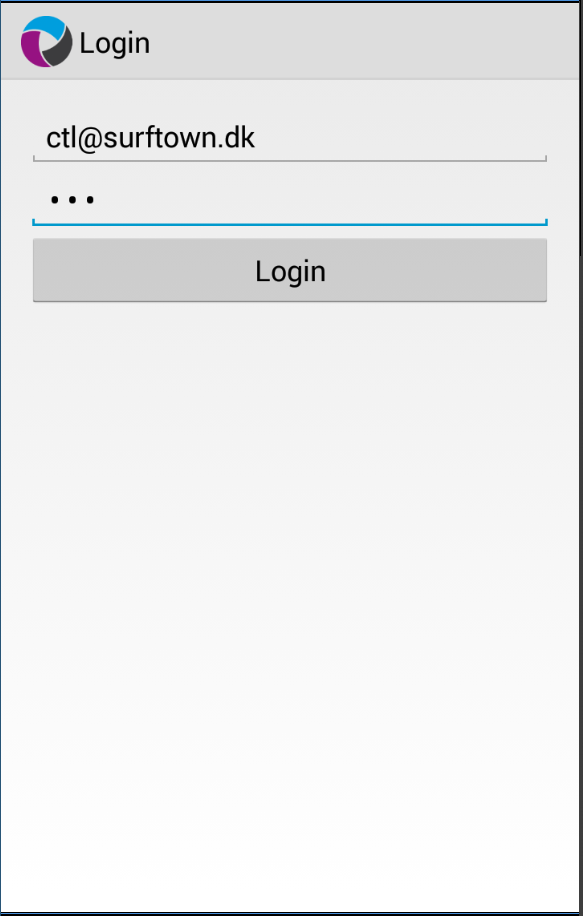
\includegraphics[width=7cm]{screenshots/login.png}
	\caption{Loginskærm på Android}
\end{figure}
\newpage
\begin{figure}[h]
	\centering
	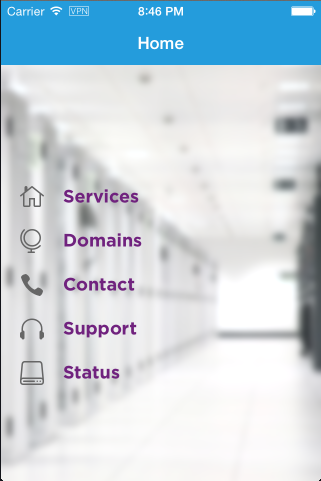
\includegraphics[width=7cm]{ios/menu.png}
	\caption{Menuskærm på iOS}
\end{figure}
\newpage
\begin{figure}[h]
	\centering
	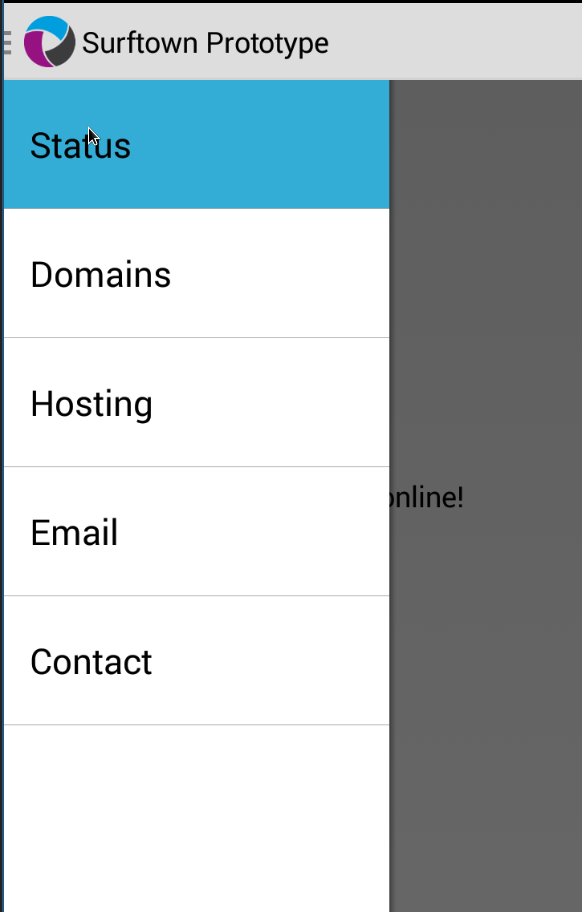
\includegraphics[width=7cm]{screenshots/menu.png}
	\caption{Menuskærm på Android}
\end{figure}
\newpage
\begin{figure}[h]
	\centering
	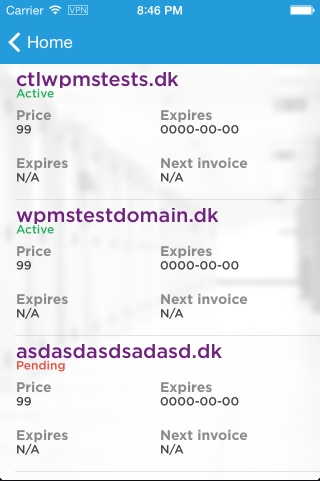
\includegraphics[width=7cm]{ios/domains.png}
	\caption{Domæneoversigtskærm på iOS}
\end{figure}
\newpage
\begin{figure}[h]
	\centering
	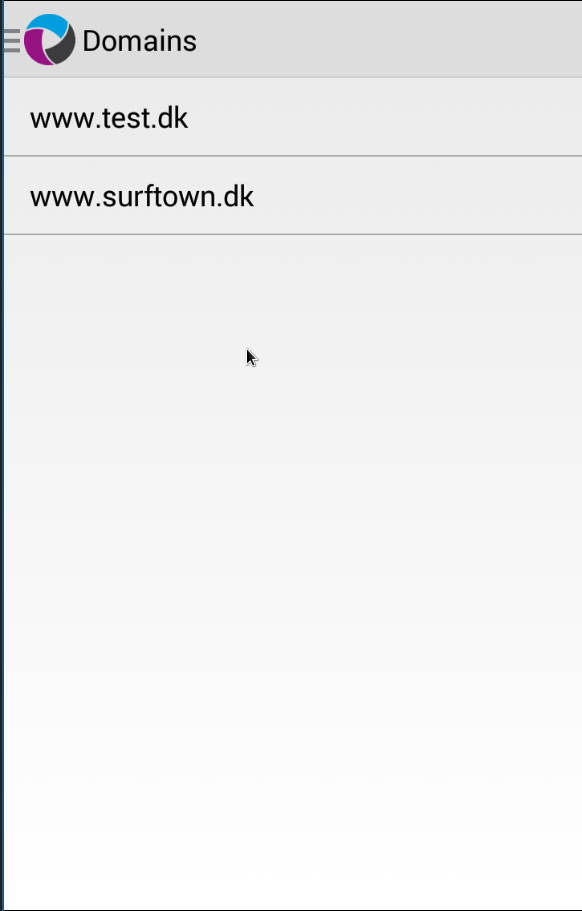
\includegraphics[width=7cm]{screenshots/domains.png}
	\caption{Domæneoversigtskærm på Android}
\end{figure}
\newpage
\subsection*{Workflow}
\begin{figure}[h]
	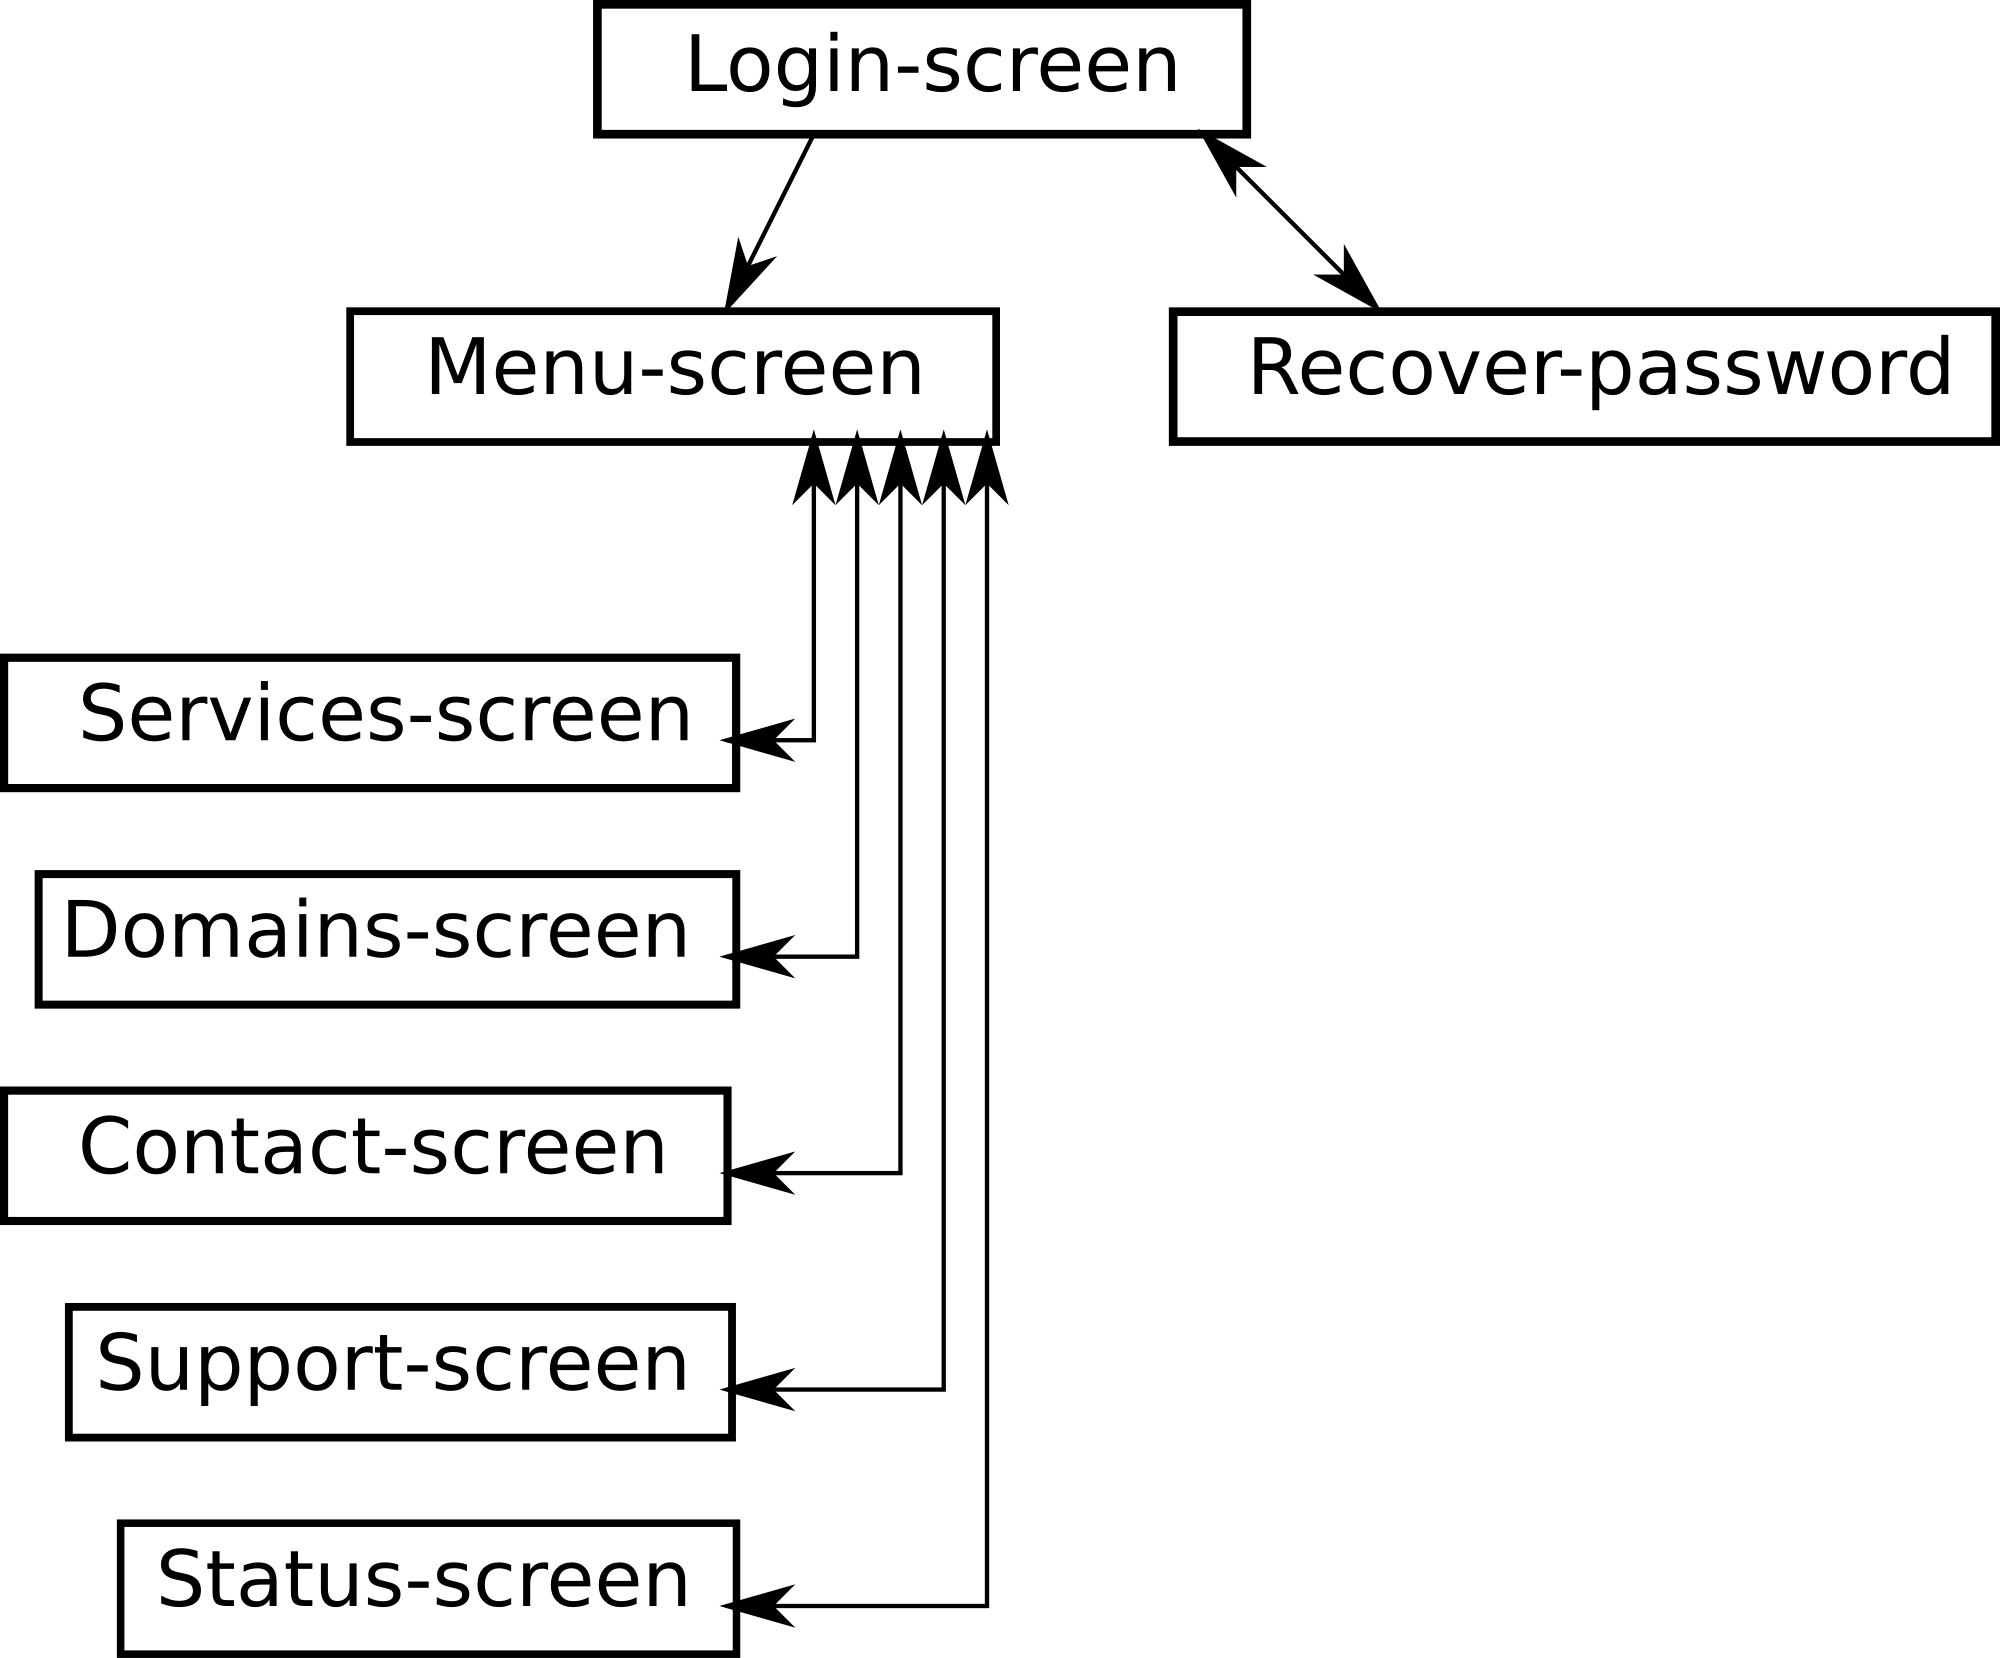
\includegraphics[width=10cm]{flow.png}
	\caption{Flowdiagram over hovedfunktionerne i Surftown applikationen}
	\label{flow}
\end{figure}
På figur \ref{flow} ses et flowdiagram over hovedfunktionerne i applikationen, hvor der tages udgangspunkt i at man kommer fra ``Login'' skærmen.
\begin{itemize}
	\item \textbf{Login-screen: } Her kan man enten logge ind i applikationen eller man kan prøve at genskabe sit password.
	\begin{itemize}
		\item \textbf{Recover-password: } Her kan man genskabe sit password og gå tilbage til ``Login'' skærmen.
		\item \textbf{Menu-screen: } Her har mulighed for at komme ind på forskellige ``views'' for at se sine oplysinger. For alle underpunkter gælder det at man kan komme tilbage til menuen for at vælge et andet ``view''.	
	\end{itemize}
\end{itemize}
\subsection{Audio-visuel præsentation}
Den audio-visuelle præsentation af prototypen, kan findes på følgende link: http://youtu.be/coaXCn-iWJE

\subsection{implementationsarbejde}

Login funktionen er valgt som eksempel, da det var den sværeste at få til at virke flydende. Når aktøren har indskrevet sin email og password og trykker på login, var det vigtigt at grænsefladen ikke gik frøs under valideringen. Derfor blev det implementeret asynkront, så aktøren får en fornemmelse af at der systemet arbejder på processen. En animation er på nuværende tidspunkt ikke implementeret. Ligeledes blev login også implementeret sådan så den automatisk kan validere en bruger i baggrunden imens applikationen starter op, så aktøren ikke skal indtaste hver gang. Dette kræver dog at password og email bliver cachet, hvilket kræver en handling og tilladelse fra brugeren.  

\newpage
\section{Systemudviklingsprocess}

\subsection{Projekt oversigt}

\begin{table}[h]
    \begin{tabular}{|l |l |l|}
	\hline
    \textbf{Begivenheder} & \textbf{Dato Fra} & \textbf{Dato Til}   \\
	\hline
    Kontakt med Surftown  & 10/2-2014 & 10/2-2014 \\
	\hline
    Første møde med Surftown & 18/2-2014 & 18/2-2014 \\
	\hline
    Analyse af Hostbill API og implementeringsmuligheder & 19/2-2014 & 16/3-2014 \\
	\hline
  Andet møde med Surftown & 17/3-2014 & 17/3-2014 \\
	\hline
    Design af Applikation og Grafisk Design & 18/3-2014 & 1/4-2014  \\
	\hline
    Implementering af prototyper  & 1/4-2014  & 1/5-2014  \\
	\hline
    Adgang til Developer Box & 1/5-2014  & 1/5-2014  \\
	\hline
    Implementering af proxy  & 1/5-2014  & 6/5-2014  \\
	\hline
    Implementering af Applikationer (Det der blev nået) & 7/5-2014  & 10/6-2014 \\
	\hline
    \end{tabular}
\caption{Skematisk oversigt over projektets fremgang fra start til slut}
\end{table}


\subsection{Forhold mellem parterne}
Surftowns marketingschef, som også fungerer som brugerrepræsentant, har oftest været meget kritisk og uformel i sine idéer og meninger omkring kravene. Der er mest blevet taget kontakt til ham og HR-chefen, hvor HR-chefen, modsat ham, har været positiv over for alle idéer, hvilket tyder på at der ikke er en fælles interesse for projektet. Udviklerne har sat fokus og mål for at appen skulle være sikker og hurtig, og har derfor ikke været så fokuserede på grafikken til at starte med. Det har skabt forvirring overfor Surftown, da de når det kommer til stykket ikke har vist interesse for andet end eye-candy, hvilket aldrig har været en del af aftalen. Udviklerne har været gode til at følge hinanden i udviklingen, og har frembragt et meget godt resultat, som der vil blive arbejdet videre på i fremtiden.

\subsection {Samarbejdet internt}
Projektgruppen har fungeret rigtig godt socialt. Der har været flere møder hvor der er blevet diskuteret, hvad der skulle laves til næste gang og hvad Surftown har kommunikeret ud\footnote{Da to medlemmer af projektgruppen arbejder hos Surftown, er det naturligvis den primære kommunikationsvej.}
Der er holdt to officielle møder med Surftown igennem projektforløbet, som ikke har været særlig effektive, da møderne har været meget ustrukturede.
Gruppen har været relativ dårlige til at strukturere arbejdet og tage referater af møderne, hvilket har medført at projektet har været lidt kaotisk. Dog skal det siges at Surftowns manglende samarbejde også har været en stor faktor for kaoset.

\subsection {Tilrettelæggelse og samspil mellem systemudviklingsaktiviteterne under projektforløb}

Systemets udvikling er dokumenteret med versionsstyresystemet Git. Det har været en styrke, under prototyping, da man hurtigt og nemt kan lave en branch, og teste noget nyt. Det var især vigtigt da problemområdet blev ændret ift. implementering af proxy-serveren. Alle API kald skulle skrives om så de fulgte et RESTful design (proxy-serveren). Det var svært at få noget konkret for anvendelsesområdet, pga besværligheden ved at installere beta-versioner af applikationer, på smartphones. Det resulterede således også i at projektdomænet kun fik foretaget en enkel user test (tænke-højt test). Det var svært at få noget konkret godt samarbejde mellem de to grupper hhv. Android og iOS, da det kun er proxy-serveren, samt kravsspecifikationen der var til fælles. Selve designet på applikationerne og implementering foregår i to forskellige perspektiver og guidelines fra hhv. Google og Apple. Dette medfører en constraint mellem de to grupper, da der rent implementeringsmæssigt ikke kunne genbruges særlig meget i form af resources eller kildekode. Der var dog en styrke, hvilket er at begge platformer gør stor brug af Model-view-controller designmønstret, hvilket gjorde at man kunne skrive den samme model, evt. i c++, som begge platforme kan kører. Den største svaghed var nok mangel på kommunikation.

\subsection {Forbedringer}
Det første og det vigtigste, er at få styr på problem- og anvendelsesområdet. Projektdomænet kan styrke sin brugeres oplevelse ved at få en klar afklaring på målsystemet. Dette kan gøres ved user tests, for at se om aktøren opfatter målsystemet efter projektdomænets opfattelse af anvendelsesområdet eller om aktøren opfatter det som et andet objektsystem, altså om aktøren har forstået, hvad målet er med systemet, eller har sin egen forståelse af systemets mål. 

%her1
\section {Review af ''Challenges of migrating to Agile methodologies'' \cite{articel} }

\subsection{Resumé}

Artiklen handler om de fordele og ulemper der er ved at skifte til "Agile" metoder. Den beskriver forudsætningerne for anvendelsen, hvilke menneskelige, organisations, process og teknisk relaterede problemer der findes og bl.a hvorfor man skal overveje at anvende metoderne. Til at starte med kommer artiklen ind på forskellen på planlægningsbaserede løsninger og Agile metoder. Den redegør derefter for hvad Agile metoder egentlig er, og dets konsekvenser, samt den internationale popularitet og tilgang til metoderne.

\subsection{Analyse og diskusion}

Artiklen nævner forskellen på Agile- og traditionelle metoder. I systemudvikling er det en god idé at bruge traditionelle metoder for nogle systemer. Artiklen nævner f.eks. at alt skal planlægges under et projekt og der bliver tildelt roller. Det ses f.eks. ved store systemer, som f.eks. Microsoft's Windows og Apple's OSX, hvor der findes projektdomæne, brugerrepræsentanter, analytikere, ingienører, driftpersonale, grafikere, ledere osv. I modsætning har vi Agile metoder, hvilket efter min opfattelse af artiklen, giver mening til mindre og ikke-risikable projekter, så som vores mobile applikation. Her har vi været flittige til at fokusere på vores kreativitet, frem for planlægning. Det ses f.eks. ved implementeringen af vores Proxy servere. Havde vi planlagt og analyserede dybere i den indledende fase, havde vi hurtigt set det sikkerhedshul, der gjorde os nødsaget til at lave proxyen. I projektgruppen findes heller ikke en leder, som tager beslutningen, men istedet foretages de i fællesskab på basis af tankegange og prototyper. Det som er væsentligt er at Agile metoder fungere i praksis til små projekter, som folk ikke er afhængige af, og som hurtigt kan opdateres, hvor den traditionelle planlægningsmetode med UML-diagrammer og OOAD\footnote{Objekt-orienteret analyse og design} skal anvendes til store API \footnote{Application programming interface} og operativsystemer. Som artiklen også nævner kan det være en god teknik at blande de to ender. Det er vigtigt at få styr på kravspecifikation, begrænsninger, kundetests og analyse af problem- og anvendelsesområde. Er der ikke foretaget disse basale steps vil man ikke vide, hvad skal laves og hvorfor. I modsætning vil man med disse informationer og aftaler kunne bruge Agile metoder efterfølgende. 

Artiklen er velskrevet og godt dokumenteret. Den er skrevet på basis af et objektivt syn på problemområderne, med en smule mere fokus på Agile metoder, hvilket giver mening, da det er grundlaget for artiklen. 

\newpage

\begin{thebibliography}{99}
\bibitem{factor} L. Mathiassen, A. Munk-Madsen, P. A. Nielsen og J. Stage.
\emph{Object-Orinted Analysis \& Design.} Marko Publishing House, 2000.
\bibitem{OOSE} B. Bruegge og A. H Dutoit.
\emph{Object-Oriented Software Engineering}
%her
\bibitem{articel} Shridhar Nerur, Radhakanta Mahapatra og George Mangalara
\emph{Challenges of migrating to Agile methodologies}

\end{thebibliography}
\section{Bilag}
\subsection{Kildekode til proxy API server}
Koden til proxy API server er vedhæftet som en zipfil med navnet proxy.zip
\subsection{Kildekode til Android applikation}
Koden til Android koden er vedhæftet som en zipfil med navnet android.zip
\subsection{Kildekoden til iOS applikationen}
iOS koden er vedhæftet som en zipfil med navnet ios.zip
\newpage
\subsection{Testspecifikationer}
\label{testSpec}
\subsubsection{RecoverPassword}
Da funktionen ``PasswordRecovery'' ikke er implementeret endnu, vil testen blive gennemført ved at vise test brugeren nogle stykker papir der viser hvordan funktionen ville se ud, hvorefter brugeren forklare hvad han/hun ville gøre.\\
        \rule{430pt}{1.0pt}
        \makebox[100pt][l]{\textbf{Mål med testen}}
        \makebox[100pt][l]{\parbox{\textwidth}{At \textbf{User} kan genskabe sit password}}\\
        \rule{430pt}{0.4pt}
        \makebox[100pt][l]{\parbox{80pt}{\textbf{Deltagende aktøre}}}
        \makebox[100pt][l]{\parbox{\textwidth}{\textbf{User}}}\\
        \rule{430pt}{0.4pt}
        \makebox[100pt][l]{\parbox{80pt}{\vspace{-200pt}\textbf{Event flow}}}
        \makebox[100pt][l]{\parbox{320pt}{
        \begin{enumerate}
          \item{\textbf{User} bliver før testen starter, fortalt at han/hun hånterer sine domæner og web hosting ved hjælp af Surftowns kontrolpanel. Han/hun skal nu bruge applikationen til at genskabe sit password}
          \item {Foran \textbf{User} bliver der fremlagt det første stykke \textbf{skærmpapir} der forestiller login-skærmen hvor der findes en ``glemt-password'' knap.}
          \item{Hvis \textbf{User} trykker på et interaktivt område i billedet så vil test manageren skifte \textbf{skærmpapir}'et til det efterfølgende skærmbillede. }
          \item{Testen afsluttes når \textbf{User} har opnået målet eller hvis \textbf{User} ikke kan komme videre.}

        \end{enumerate}
        }}\\
\newpage
\subsubsection{Login- og navigationstest}
Denne test kan udføres igennem en iOS simulator.\\
        \rule{430pt}{1.0pt}
        \makebox[100pt][l]{\textbf{Mål med testen}}
        \makebox[100pt][l]{\parbox{\textwidth}{At \textbf{User} kan logge ind \\ At \textbf{User} kan finde sine hosting services
                                                        \\ At \textbf{User} kan finde sine registrerede domæner}}\\
        \rule{430pt}{0.4pt}
        \makebox[100pt][l]{\parbox{80pt}{\textbf{Deltagende aktøre}}}
        \makebox[100pt][l]{\parbox{\textwidth}{\textbf{User}}}\\
        \rule{430pt}{0.4pt}
        \makebox[100pt][l]{\parbox{80pt}{\vspace{-170pt}\textbf{Event flow}}}
        \makebox[100pt][l]{\parbox{320pt}{
        \begin{enumerate}
	  \item{\textbf{User} bliver fortalt, at han/hun håndterer sine domæner og web hosting ved hjælp af Surftowns kontrolpanel. Han/hun skal nu bruge applikationen til at logge ind for at finde sine domæner og services}
          \item {Foran \textbf{User} bliver der sat en computer med en iOS simulator kørende og login-skærmen er blevet initialiseret.}
          \item{Via musen på computeren kan \textbf{User} navigere og interagere med applikationen.}
          \item{Testen afsluttes når \textbf{User} har opnået målet eller hvis \textbf{User} ikke kan komme videre.}
          
        \end{enumerate}
        }}\\
\newpage

\end{document}
